% !TeX program = xelatex
% !TeX encoding = UTF-8
\RequirePackage{iftex}
\ifPDFTeX
\errmessage{This Vietnamese report requires XeLaTeX. Select the XeLaTeX recipe or run latexmk -xelatex report.tex}
\expandafter\endinput
\fi
% Options for packages loaded elsewhere
\PassOptionsToPackage{unicode}{hyperref}
\PassOptionsToPackage{hyphens}{url}
\PassOptionsToPackage{dvipsnames,svgnames,x11names}{xcolor}
%
\documentclass[
  11pt,
]{article}
\usepackage{amsmath,amssymb}
\usepackage{setspace}
\usepackage{iftex}
\ifPDFTeX
  \usepackage[T1]{fontenc}
  \usepackage[utf8]{inputenc}
  \usepackage{textcomp} % provide euro and other symbols
\else % if luatex or xetex
  \usepackage{unicode-math} % this also loads fontspec
  \defaultfontfeatures{Scale=MatchLowercase}
  \defaultfontfeatures[\rmfamily]{Ligatures=TeX,Scale=1}
\fi
\usepackage{lmodern}
\ifPDFTeX\else
  % xetex/luatex font selection
\fi
% Use upquote if available, for straight quotes in verbatim environments
\IfFileExists{upquote.sty}{\usepackage{upquote}}{}
\IfFileExists{microtype.sty}{% use microtype if available
  \usepackage[]{microtype}
  \UseMicrotypeSet[protrusion]{basicmath} % disable protrusion for tt fonts
}{}
\makeatletter
\@ifundefined{KOMAClassName}{% if non-KOMA class
  \IfFileExists{parskip.sty}{%
    \usepackage{parskip}
  }{% else
    \setlength{\parindent}{0pt}
    \setlength{\parskip}{6pt plus 2pt minus 1pt}}
}{% if KOMA class
  \KOMAoptions{parskip=half}}
\makeatother
\usepackage{xcolor}
\usepackage[a4paper,margin=22mm]{geometry}
\usepackage{color}
\usepackage{fancyvrb}
\newcommand{\VerbBar}{|}
\newcommand{\VERB}{\Verb[commandchars=\\\{\}]}
\DefineVerbatimEnvironment{Highlighting}{Verbatim}{commandchars=\\\{\}}
% Add ',fontsize=\small' for more characters per line
\newenvironment{Shaded}{}{}
\newcommand{\AlertTok}[1]{\textcolor[rgb]{1.00,0.00,0.00}{\textbf{#1}}}
\newcommand{\AnnotationTok}[1]{\textcolor[rgb]{0.38,0.63,0.69}{\textbf{\textit{#1}}}}
\newcommand{\AttributeTok}[1]{\textcolor[rgb]{0.49,0.56,0.16}{#1}}
\newcommand{\BaseNTok}[1]{\textcolor[rgb]{0.25,0.63,0.44}{#1}}
\newcommand{\BuiltInTok}[1]{\textcolor[rgb]{0.00,0.50,0.00}{#1}}
\newcommand{\CharTok}[1]{\textcolor[rgb]{0.25,0.44,0.63}{#1}}
\newcommand{\CommentTok}[1]{\textcolor[rgb]{0.38,0.63,0.69}{\textit{#1}}}
\newcommand{\CommentVarTok}[1]{\textcolor[rgb]{0.38,0.63,0.69}{\textbf{\textit{#1}}}}
\newcommand{\ConstantTok}[1]{\textcolor[rgb]{0.53,0.00,0.00}{#1}}
\newcommand{\ControlFlowTok}[1]{\textcolor[rgb]{0.00,0.44,0.13}{\textbf{#1}}}
\newcommand{\DataTypeTok}[1]{\textcolor[rgb]{0.56,0.13,0.00}{#1}}
\newcommand{\DecValTok}[1]{\textcolor[rgb]{0.25,0.63,0.44}{#1}}
\newcommand{\DocumentationTok}[1]{\textcolor[rgb]{0.73,0.13,0.13}{\textit{#1}}}
\newcommand{\ErrorTok}[1]{\textcolor[rgb]{1.00,0.00,0.00}{\textbf{#1}}}
\newcommand{\ExtensionTok}[1]{#1}
\newcommand{\FloatTok}[1]{\textcolor[rgb]{0.25,0.63,0.44}{#1}}
\newcommand{\FunctionTok}[1]{\textcolor[rgb]{0.02,0.16,0.49}{#1}}
\newcommand{\ImportTok}[1]{\textcolor[rgb]{0.00,0.50,0.00}{\textbf{#1}}}
\newcommand{\InformationTok}[1]{\textcolor[rgb]{0.38,0.63,0.69}{\textbf{\textit{#1}}}}
\newcommand{\KeywordTok}[1]{\textcolor[rgb]{0.00,0.44,0.13}{\textbf{#1}}}
\newcommand{\NormalTok}[1]{#1}
\newcommand{\OperatorTok}[1]{\textcolor[rgb]{0.40,0.40,0.40}{#1}}
\newcommand{\OtherTok}[1]{\textcolor[rgb]{0.00,0.44,0.13}{#1}}
\newcommand{\PreprocessorTok}[1]{\textcolor[rgb]{0.74,0.48,0.00}{#1}}
\newcommand{\RegionMarkerTok}[1]{#1}
\newcommand{\SpecialCharTok}[1]{\textcolor[rgb]{0.25,0.44,0.63}{#1}}
\newcommand{\SpecialStringTok}[1]{\textcolor[rgb]{0.73,0.40,0.53}{#1}}
\newcommand{\StringTok}[1]{\textcolor[rgb]{0.25,0.44,0.63}{#1}}
\newcommand{\VariableTok}[1]{\textcolor[rgb]{0.10,0.09,0.49}{#1}}
\newcommand{\VerbatimStringTok}[1]{\textcolor[rgb]{0.25,0.44,0.63}{#1}}
\newcommand{\WarningTok}[1]{\textcolor[rgb]{0.38,0.63,0.69}{\textbf{\textit{#1}}}}
\usepackage{longtable,booktabs,array,tabularx}
\usepackage{calc} % for calculating minipage widths
% Correct order of tables after \paragraph or \subparagraph
\usepackage{etoolbox}
\makeatletter
\patchcmd\longtable{\par}{\if@noskipsec\mbox{}\fi\par}{}{}
\makeatother
% Allow footnotes in longtable head/foot
\IfFileExists{footnotehyper.sty}{\usepackage{footnotehyper}}{\usepackage{footnote}}
\makesavenoteenv{longtable}
\usepackage{graphicx}
\makeatletter
\def\maxwidth{\ifdim\Gin@nat@width>\linewidth\linewidth\else\Gin@nat@width\fi}
\def\maxheight{\ifdim\Gin@nat@height>\textheight\textheight\else\Gin@nat@height\fi}
\makeatother
% Scale images if necessary, so that they will not overflow the page
% margins by default, and it is still possible to overwrite the defaults
% using explicit options in \includegraphics[width, height, ...]{}
\setkeys{Gin}{width=\maxwidth,height=\maxheight,keepaspectratio}
% Set default figure placement to htbp
\makeatletter
\def\fps@figure{htbp}
\makeatother
\setlength{\emergencystretch}{3em} % prevent overfull lines
\providecommand{\tightlist}{%
  \setlength{\itemsep}{0pt}\setlength{\parskip}{0pt}}
\setcounter{secnumdepth}{5}
\usepackage{fancyhdr}
\usepackage{microtype}
\usepackage{xurl}
\usepackage{tikz}
\usepackage{etoolbox}
\usepackage{needspace}
\usepackage{caption}
\usepackage{placeins}
\usepackage{pdflscape}
% Unicode fonts available both in a normal TeX Live install and on Windows.
% No dependency on Microsoft fonts on Linux or Overleaf.
\IfFontExistsTF{TeX Gyre Termes}{\setmainfont{TeX Gyre Termes}}{\setmainfont{DejaVu Serif}}
\IfFontExistsTF{TeX Gyre Heros}{\setsansfont{TeX Gyre Heros}}{\setsansfont{DejaVu Sans}}
\IfFontExistsTF{Consolas}{\setmonofont{Consolas}[Scale=MatchLowercase]}{\IfFontExistsTF{DejaVu Sans Mono}{\setmonofont{DejaVu Sans Mono}[Scale=MatchLowercase]}{\setmonofont{TeX Gyre Cursor}[Scale=MatchLowercase]}}

\PassOptionsToPackage{pdflang=vi-VN}{hyperref}
\usetikzlibrary{calc}
% Thông tin bìa có thể sửa trực tiếp; dùng UTF-8 và biên dịch bằng XeLaTeX.
\newcommand{\ReportUniversity}{ĐẠI HỌC QUỐC GIA THÀNH PHỐ HỒ CHÍ MINH}
\newcommand{\ReportSchool}{TRƯỜNG ĐẠI HỌC BÁCH KHOA}
\newcommand{\ReportCourse}{Mạng máy tính}
\newcommand{\ReportTitle}{THIẾT KẾ VÀ MÔ PHỎNG\\[2mm]MẠNG BỆNH VIỆN BA CƠ SỞ}
\newcommand{\ReportSubtitle}{Main -- Điện Biên Phủ -- Bà Huyện Thanh Quan}
\newcommand{\ReportTeam}{Dự án BTL Computer Network}
\newcommand{\ReportLecturer}{}
\newcommand{\ReportClass}{}
% Có thể dùng \begin{tabular}...\end{tabular} để ghi họ tên và MSSV.
\newcommand{\ReportMembers}{}
\newcommand{\ReportPlaceDate}{Thành phố Hồ Chí Minh, tháng 11 năm 2026}

\definecolor{BKBlue}{HTML}{082F87}
\definecolor{BKLightBlue}{HTML}{1489D4}
\renewcommand{\contentsname}{Mục lục}
\renewcommand{\listfigurename}{Danh mục hình ảnh}
\renewcommand{\listtablename}{Danh mục bảng biểu}
\renewcommand{\refname}{Tài liệu tham khảo}
\captionsetup{font=small,labelfont=bf,labelsep=colon,skip=5pt,hypcap=false}
\captionsetup[table]{position=top}
\newcommand{\tabletitle}[1]{\par\begingroup\captionof{table}{#1}\endgroup\nopagebreak}
\renewcommand{\figurename}{Hình}
\renewcommand{\tablename}{Bảng}
\pagestyle{fancy}
\fancyhf{}
\fancyhead[L]{\small BTL 2 | Mạng máy tính}
\fancyhead[R]{\small Main / DBP / BHTQ}
\fancyfoot[C]{\thepage}
\setlength{\headheight}{16pt}
\setlength{\emergencystretch}{3em}
\clubpenalty=10000
\widowpenalty=10000
\renewcommand{\arraystretch}{1.2}
\makeatletter
\renewcommand*\l@subsection{\@dottedtocline{2}{1.5em}{3.4em}}
\makeatother
\fancypagestyle{plain}{\fancyhf{}\renewcommand{\headrulewidth}{0pt}\fancyfoot[C]{\thepage}}
\let\originaltableofcontents\tableofcontents
\renewcommand{\tableofcontents}{%
  \clearpage\pagestyle{plain}\begingroup\footnotesize\setstretch{1}\originaltableofcontents\endgroup
  \clearpage}
\AtBeginDocument{\hypersetup{
  pdftitle={Thiết kế và mô phỏng mạng bệnh viện ba cơ sở},
  pdfauthor={\ReportTeam},
  pdfsubject={Báo cáo bài tập lớn 2 - Mạng máy tính}}}

\ifLuaTeX
  \usepackage{selnolig}  % disable illegal ligatures
\fi
\IfFileExists{bookmark.sty}{\usepackage{bookmark}}{\usepackage{hyperref}}
\IfFileExists{xurl.sty}{\usepackage{xurl}}{} % add URL line breaks if available
\urlstyle{same}
\hypersetup{
  colorlinks=true,
  linkcolor={BKBlue},
  filecolor={Maroon},
  citecolor={Blue},
  urlcolor={BKBlue},
  pdfcreator={LaTeX via pandoc}}

\author{}
\date{}

\newcommand{\pic}[3]{\par\medskip\begin{center}\includegraphics[width=\linewidth,height=#2,keepaspectratio]{#1}\captionof{figure}{#3}\end{center}\medskip}

\begin{document}
\begin{titlepage}
\thispagestyle{empty}
\begin{tikzpicture}[remember picture,overlay]
  \draw[BKBlue,line width=0.9pt]
    ([xshift=15mm,yshift=-15mm]current page.north west)
    rectangle ([xshift=-15mm,yshift=15mm]current page.south east);
\end{tikzpicture}
\centering
\vspace*{3mm}
{\fontsize{12}{17}\selectfont\ReportUniversity\par}
\vspace{2mm}
{\fontsize{15}{20}\selectfont\bfseries\ReportSchool\par}
\vspace{3mm}
{\color{BKBlue}\rule{65mm}{0.6pt}\par}
\vspace{13mm}
% Giữ nguyên PNG người dùng cung cấp. Chỉ cắt vùng trong suốt khi dàn trang.
% Ảnh 3509x2481 px, 300 dpi; alpha bbox (1078,233)-(2822,2007).

\includegraphics[width=38mm,trim={258.72bp 113.76bp 164.88bp 55.92bp},clip]{assets/logo-bach-khoa.png}\par
\vspace{13mm}
{\fontsize{16}{21}\selectfont\bfseries BÁO CÁO BÀI TẬP LỚN 2\par}
\vspace{3mm}
{\large Môn học: \ReportCourse\par}
\vspace{12mm}
{\color{BKBlue}\fontsize{21}{29}\selectfont\bfseries\ReportTitle\par}
\vspace{5mm}
{\fontsize{12}{18}\selectfont\ReportSubtitle\par}
\vspace{9mm}
\begin{minipage}{0.82\textwidth}
  \setlength{\parskip}{2mm}
  \textbf{Nhóm thực hiện:} \ReportTeam\par
  \ifdefempty{\ReportLecturer}{}{\textbf{Giảng viên hướng dẫn:} \ReportLecturer\par}
  \ifdefempty{\ReportClass}{}{\textbf{Lớp:} \ReportClass\par}
  \ifdefempty{\ReportMembers}{}{\textbf{Thực hiện BTL2:}\par\ReportMembers\par}
\end{minipage}
\vfill
{\fontsize{12}{17}\selectfont\ReportPlaceDate\par}
\vspace*{5mm}
\end{titlepage}

\clearpage
\thispagestyle{empty}

\begin{center}
\renewcommand{\arraystretch}{1.3}
\begin{tabular}{|c|l|c|l|c|}
\hline
\textbf{STT} & \textbf{Họ và tên} & \textbf{MSSV} & \textbf{Email sinh viên} & \textbf{Phân công} \\
\hline
1 & Nguyễn Thành Đạt & 2410709 & \url{dat.nguyen19052006@hcmut.edu.vn} & BTL2 \\
\hline
2 & Nguyễn Phúc Bảo Đạt & 2410696 & \url{dat.nguyen662006@hcmut.edu.vn} & BTL1 \\
\hline
3 & Bùi Công Danh & 2410448 & \url{danh.buicong@hcmut.edu.vn} & BTL1 \\
\hline
4 & Nguyễn Minh Đạt & 2410694 & \url{dat.nguyen2410694@hcmut.edu.vn} & BTL1 \\
\hline
5 & Phạm Tiến Đạt & 2410723 & \url{dat.pham123qwe@hcmut.edu.vn} & BTL2 \\
\hline
\end{tabular}
\end{center}

\vfill
\clearpage
\pagenumbering{roman}

\setcounter{tocdepth}{2}
\tableofcontents
\phantomsection
\addcontentsline{toc}{section}{Danh mục hình ảnh}
\listoffigures
\clearpage
\phantomsection
\addcontentsline{toc}{section}{Danh mục bảng biểu}
\listoftables
\clearpage
\pagenumbering{arabic}
\pagestyle{fancy}
\setstretch{1.08}
\section{Giới thiệu và khảo sát (Step 1)}
\subsection{Yêu cầu và phạm vi}
Bệnh viện gồm Main tại TP.HCM và hai cơ sở DBP, BHTQ. Hệ thống phải phục vụ nghiệp vụ khám chữa bệnh, truy cập máy chủ tập trung, Internet và khách không dây. Mục tiêu là chuyển đặc tả thành kiến trúc có thể kiểm chứng, có dự phòng dung lượng và ranh giới bảo mật rõ ràng.
\par\noindent
\tabletitle{Quy mô và yêu cầu tại ba cơ sở}
\begin{tabularx}{\linewidth}{@{}lXXX@{}}\toprule
Thông số & Main & DBP & BHTQ\\\midrule
Công trình & Hai tòa, mỗi tòa 5 tầng, 10 phòng/tầng & Một tòa 2 tầng & Một tòa 2 tầng\\
Máy trạm & 600 & 260 & 260\\
Server ứng dụng & 10 & 2 & 2\\
Sau 5 năm & 720 PC, 12 server & 312 PC, 3 server & 312 PC, 3 server\\
Hạ tầng & DC riêng cách khoảng 50 m; hai ISP & Một leased line về Main & Một leased line về Main\\\bottomrule\end{tabularx}\par

Tăng trưởng là 20\% tổng trong 5 năm. Số server phải làm tròn nguyên. Số thiết bị mạng minh họa trong đề không phải giới hạn cứng khi tính cổng cho 1.120 PC. Main có DC tách khỏi hai tòa; chiều dài cáp phải đo theo tuyến thực tế, không lấy khoảng cách thẳng 50 m thay cho toàn bộ tuyến.

\textbf{Phạm vi xác nhận.} Dự án chọn Cisco Packet Tracer làm nền tảng mô phỏng duy nhất. Thiết kế gồm BOM, địa chỉ, GPON, Wi-Fi, camera và VPN; kiểm thử chức năng dựa trên native và raw output Cisco. Các chức năng chưa có bằng chứng trên Packet Tracer tiếp tục được ghi là đề xuất hoặc chưa kiểm chứng.

Yêu cầu thiết kế được xác định từ đặc tả bài tập lớn \cite{assignment}; các giả định bổ sung được nêu tại từng nội dung liên quan.

\clearpage
\subsection{Khảo sát, khu vực tải cao và tiêu chí nghiệm thu}
Các phân bố khoa/phòng, số AP và camera là giả định quy hoạch. Trước thi công cần xác nhận các đầu vào dưới đây với bệnh viện; không coi bản vẽ mô phỏng là biên bản khảo sát thực địa.
\par\noindent
\tabletitle{Nội dung khảo sát và đầu ra kiểm nhận}
\begin{tabularx}{\linewidth}{@{}p{.19\linewidth}XX@{}}\toprule
Nhóm & Cần thu thập & Đầu ra kiểm nhận\\\midrule
Nghiệp vụ & HIS/LIS/PACS, giờ cao điểm, số phiên, mức ưu tiên & Ma trận nguồn--đích, SLA và tải ứng dụng\\
Mặt bằng & Vị trí phòng, DC, MDF/IDF, tuyến A/B & Sơ đồ rack, cáp, ODF và khoảng cách\\
Điện/điều hòa & UPS, tiếp địa, tải PoE, thời gian lưu điện & Bảng tải và thử mất nguồn\\
Wi-Fi & Vật cản, vùng phủ, thiết bị đồng thời, nhiễu & RF survey trước/sau và vị trí AP\\
Camera & Góc nhìn, vùng riêng tư, bitrate, thời gian lưu & Sơ đồ camera, quyền xem và sizing NVR\\
Nhà mạng & Handoff, hai chiều, SLA, tuyến vật lý & Báo giá cùng phạm vi và phương án lỗi\\
An toàn & Quyền truy cập, tài khoản, log, backup & Ma trận ACL, quy trình đổi cấu hình/khôi phục\\\bottomrule\end{tabularx}\par

\textbf{Xác định khu vực tải cao.} Đề yêu cầu xác định vùng tải cao để chọn cấu hình thiết bị và đặt cân bằng tải tại nơi cần thiết. Ưu tiên xem xét Internet Edge/FW tại Main, WAN Aux--Main, Server Farm/PACS, uplink tầng, Wi-Fi đông khách và NVR cục bộ. Mục \ref{sec:highload} đối chiếu tải, giới hạn và biện pháp cho từng vùng; tải cao không tự chứng minh đang nghẽn. HIS/LIS cần ưu tiên độ trễ hơn backup/khách; video ghi local không mặc nhiên đi WAN.

\textbf{Điều kiện chốt thiết kế.} Xác nhận số thiết bị theo tầng, tỷ lệ LAN/WAN/Internet, số khách theo ngày và đồng thời, thời gian lưu video, tải thiết yếu khi mất ISP, model/license/nguồn và báo giá. Những điều kiện này là phần nghiệm thu triển khai còn mở.

Bảng truy vết ở phụ lục đối chiếu bảy bước của đặc tả với nội dung và giới hạn nghiệm thu trong báo cáo.

\clearpage
\subsection{Kiến trúc và luồng nghiệp vụ}
Main tách các chức năng core, phân phối và access; Aux dùng collapsed core phù hợp quy mô. Kiến trúc triển khai đề xuất có hai core, uplink độc lập và firewall kiểm soát DMZ. Native lab dùng số node đại diện nên không chứng minh HA chassis.
\pic{assets/layers-cisco.pdf}{.42\textheight}{Các chức năng phân tầng đề xuất cho Main và Aux.}
\par\noindent
\tabletitle{Luồng nghiệp vụ và điểm kiểm soát}
\begin{tabularx}{\linewidth}{@{}lXX@{}}\toprule
Luồng & Đường đi & Kiểm soát chính\\\midrule
PC Main--HIS & Access--Core--Server Farm & VLAN vai trò, ACL và quyền ứng dụng\\
Aux--HIS & Aux-GW--WAN--Main--Farm & OSPF, route phản hồi và ACL\\
Ba site--Internet & Gateway--Main-FW--Edge--ISP & Chính sách tập trung, PAT và DNS\\
Guest & VLAN 100--Main--Internet & Chặn nội bộ, vẫn có DHCP/DNS/Web\\
Camera & VLAN 110--NVR cùng site & Quyền xem riêng, không publish Internet\\\bottomrule\end{tabularx}\par

VLAN 70 chứa Server Farm; DMZ 80 kết thúc tại firewall. Quản trị VLAN 90, Guest 100, camera 110 và Staff 120 tách riêng. Không kéo broadcast lớp 2 xuyên leased line. Một giao dịch liên site cần xét cả chiều đi, chiều trả lời và vị trí áp chính sách.

\clearpage
\section{Thiết kế hạ tầng (Step 2)}
\subsection{Ngân sách cổng và tăng trưởng}
PC phân bổ đều để lập ngân sách ban đầu: Main 60 PC/tầng, mỗi Aux 130 PC/tầng. Dự trù 3 AP và 4 camera/tầng; sau tăng trưởng làm tròn lên 4 AP và 5 camera/tầng. Cần điều chỉnh sau khảo sát thay vì xem đây là số lượng RF đã đo.
\par\noindent
\tabletitle{Ngân sách cổng hiện tại và sau năm năm}
\begin{tabularx}{\linewidth}{@{}lXXX@{}}\toprule
Hạng mục & Main & DBP & BHTQ\\\midrule
Access 48 cổng & 20 / 960 cổng & 8 / 384 cổng & 8 / 384 cổng\\
PC hiện tại / 5 năm & 600 / 720 & 260 / 312 & 260 / 312\\
AP hiện tại / 5 năm & 30 / 40 & 6 / 8 & 6 / 8\\
Camera hiện tại / 5 năm & 40 / 50 & 8 / 10 & 8 / 10\\
Server trên access & 0 / 0 & 2 / 3 & 2 / 3\\
NVR trên access & 0 & 1 & 1\\
Cổng dùng hiện tại & 670 & 277 & 277\\
Cổng dùng sau 5 năm & 810 & 334 & 334\\
Cổng dư sau 5 năm & 150 & 50 & 50\\\bottomrule\end{tabularx}\par

Main cần mỗi tầng 2 switch: $72+4+5=81/96$ cổng ở năm thứ 5. Aux có 4 switch/tầng: tầng 1 dùng tối đa $156+4+5+3+1=169/192$ cổng; tầng 2 dùng $165/192$. Main đặt server và NVR trên switch Server Farm riêng nên không cộng lại vào access campus.

Dư cổng toàn site không bảo đảm dự phòng cho máy đang nối vào một switch hỏng. Cần chia nhóm nghiệp vụ và AP/camera giữa các switch, có cổng dự phòng tại đúng IDF, không chỉ trên bảng tổng.

Mô hình Packet Tracer dùng thiết bị đại diện; số lượng trong mô phỏng không thay thế ngân sách thiết bị triển khai.

\clearpage
\subsection{Thiết bị chủ chốt và PoE}
\par\noindent
\tabletitle{Thiết bị chủ chốt tại Main và các cơ sở phụ}
\begin{tabularx}{\linewidth}{@{}lXX@{}}\toprule
Thành phần & Main & Mỗi Aux\\\midrule
Core / distribution & 2 core L3, liên kết 40 G & 2 collapsed core L3\\
Access & 20 switch 48\,$\times$\,1 G, uplink 10 G & 8 switch tương tự\\
Server Farm & 2 switch, $\ge24\times10$ G mỗi switch & Server cục bộ trên access\\
DMZ & 2 switch sau firewall & Không có DMZ công bố riêng\\
WAN / firewall & Router WAN, Internet Edge; cặp FW đề xuất & CPE WAN và chính sách tại GW\\
Wi-Fi / NVR & 30 AP; NVR $\ge64$ kênh & 6 AP; NVR $\ge16$ kênh\\\bottomrule\end{tabularx}\par

\textbf{PoE.} Giả định PSE 30 W/AP, 15,4 W/camera. Một tầng hiện tại cần $3\times30+4\times15,4=151,6$ W; sau 5 năm cần $4\times30+5\times15,4=197$ W. C9200L-48P-4X với PSU 1 kW có ngân sách PoE 740 W theo datasheet Cisco \cite{c9200}; không nhầm với bản 48PL/nguồn 600 W có 370 W. Phải kiểm từng switch và điều kiện mất PSU; tổng công suất toàn tầng chưa xác nhận HA nguồn.

AP 9115AXI có uplink đến 2,5 GbE \cite{c9115} nhưng access baseline chỉ 1 GbE. Nâng mGig kéo theo switch, PoE và BOM. Tổng AP hiện tại 42, dự trù 56; mỗi WLC dự phòng cần capacity ít nhất 64 AP nếu nhận toàn bộ tải khi một WLC lỗi. Đây là yêu cầu lựa chọn, chưa có thử WLC failover.

Hai switch Server Farm cần stack/MLAG phù hợp trước khi ghép LACP qua hai chassis \cite{etherchannel}; nếu không, dùng NIC active/standby theo thiết kế. Mỗi switch Farm dự trù 15/24 cổng ở năm thứ 5 gồm server NIC, NVR, core và inter-switch. Firewall HA, license và uplink phải xác nhận theo model thực.

Giá chưa chốt; số model là tham chiếu năng lực, không phải thiết bị đã mua.

\clearpage
\subsection{Mặt bằng, MDF/IDF và tuyến cáp}
Main có MDF/DC riêng; mỗi tầng hai tòa có IDF. Mỗi Aux đặt MDF tầng 1 và IDF tầng 2. Cáp đồng tới máy trạm/AP/camera; backbone quang theo hai tuyến A/B, tránh chung điểm cắt nếu có điều kiện.
\begin{center}
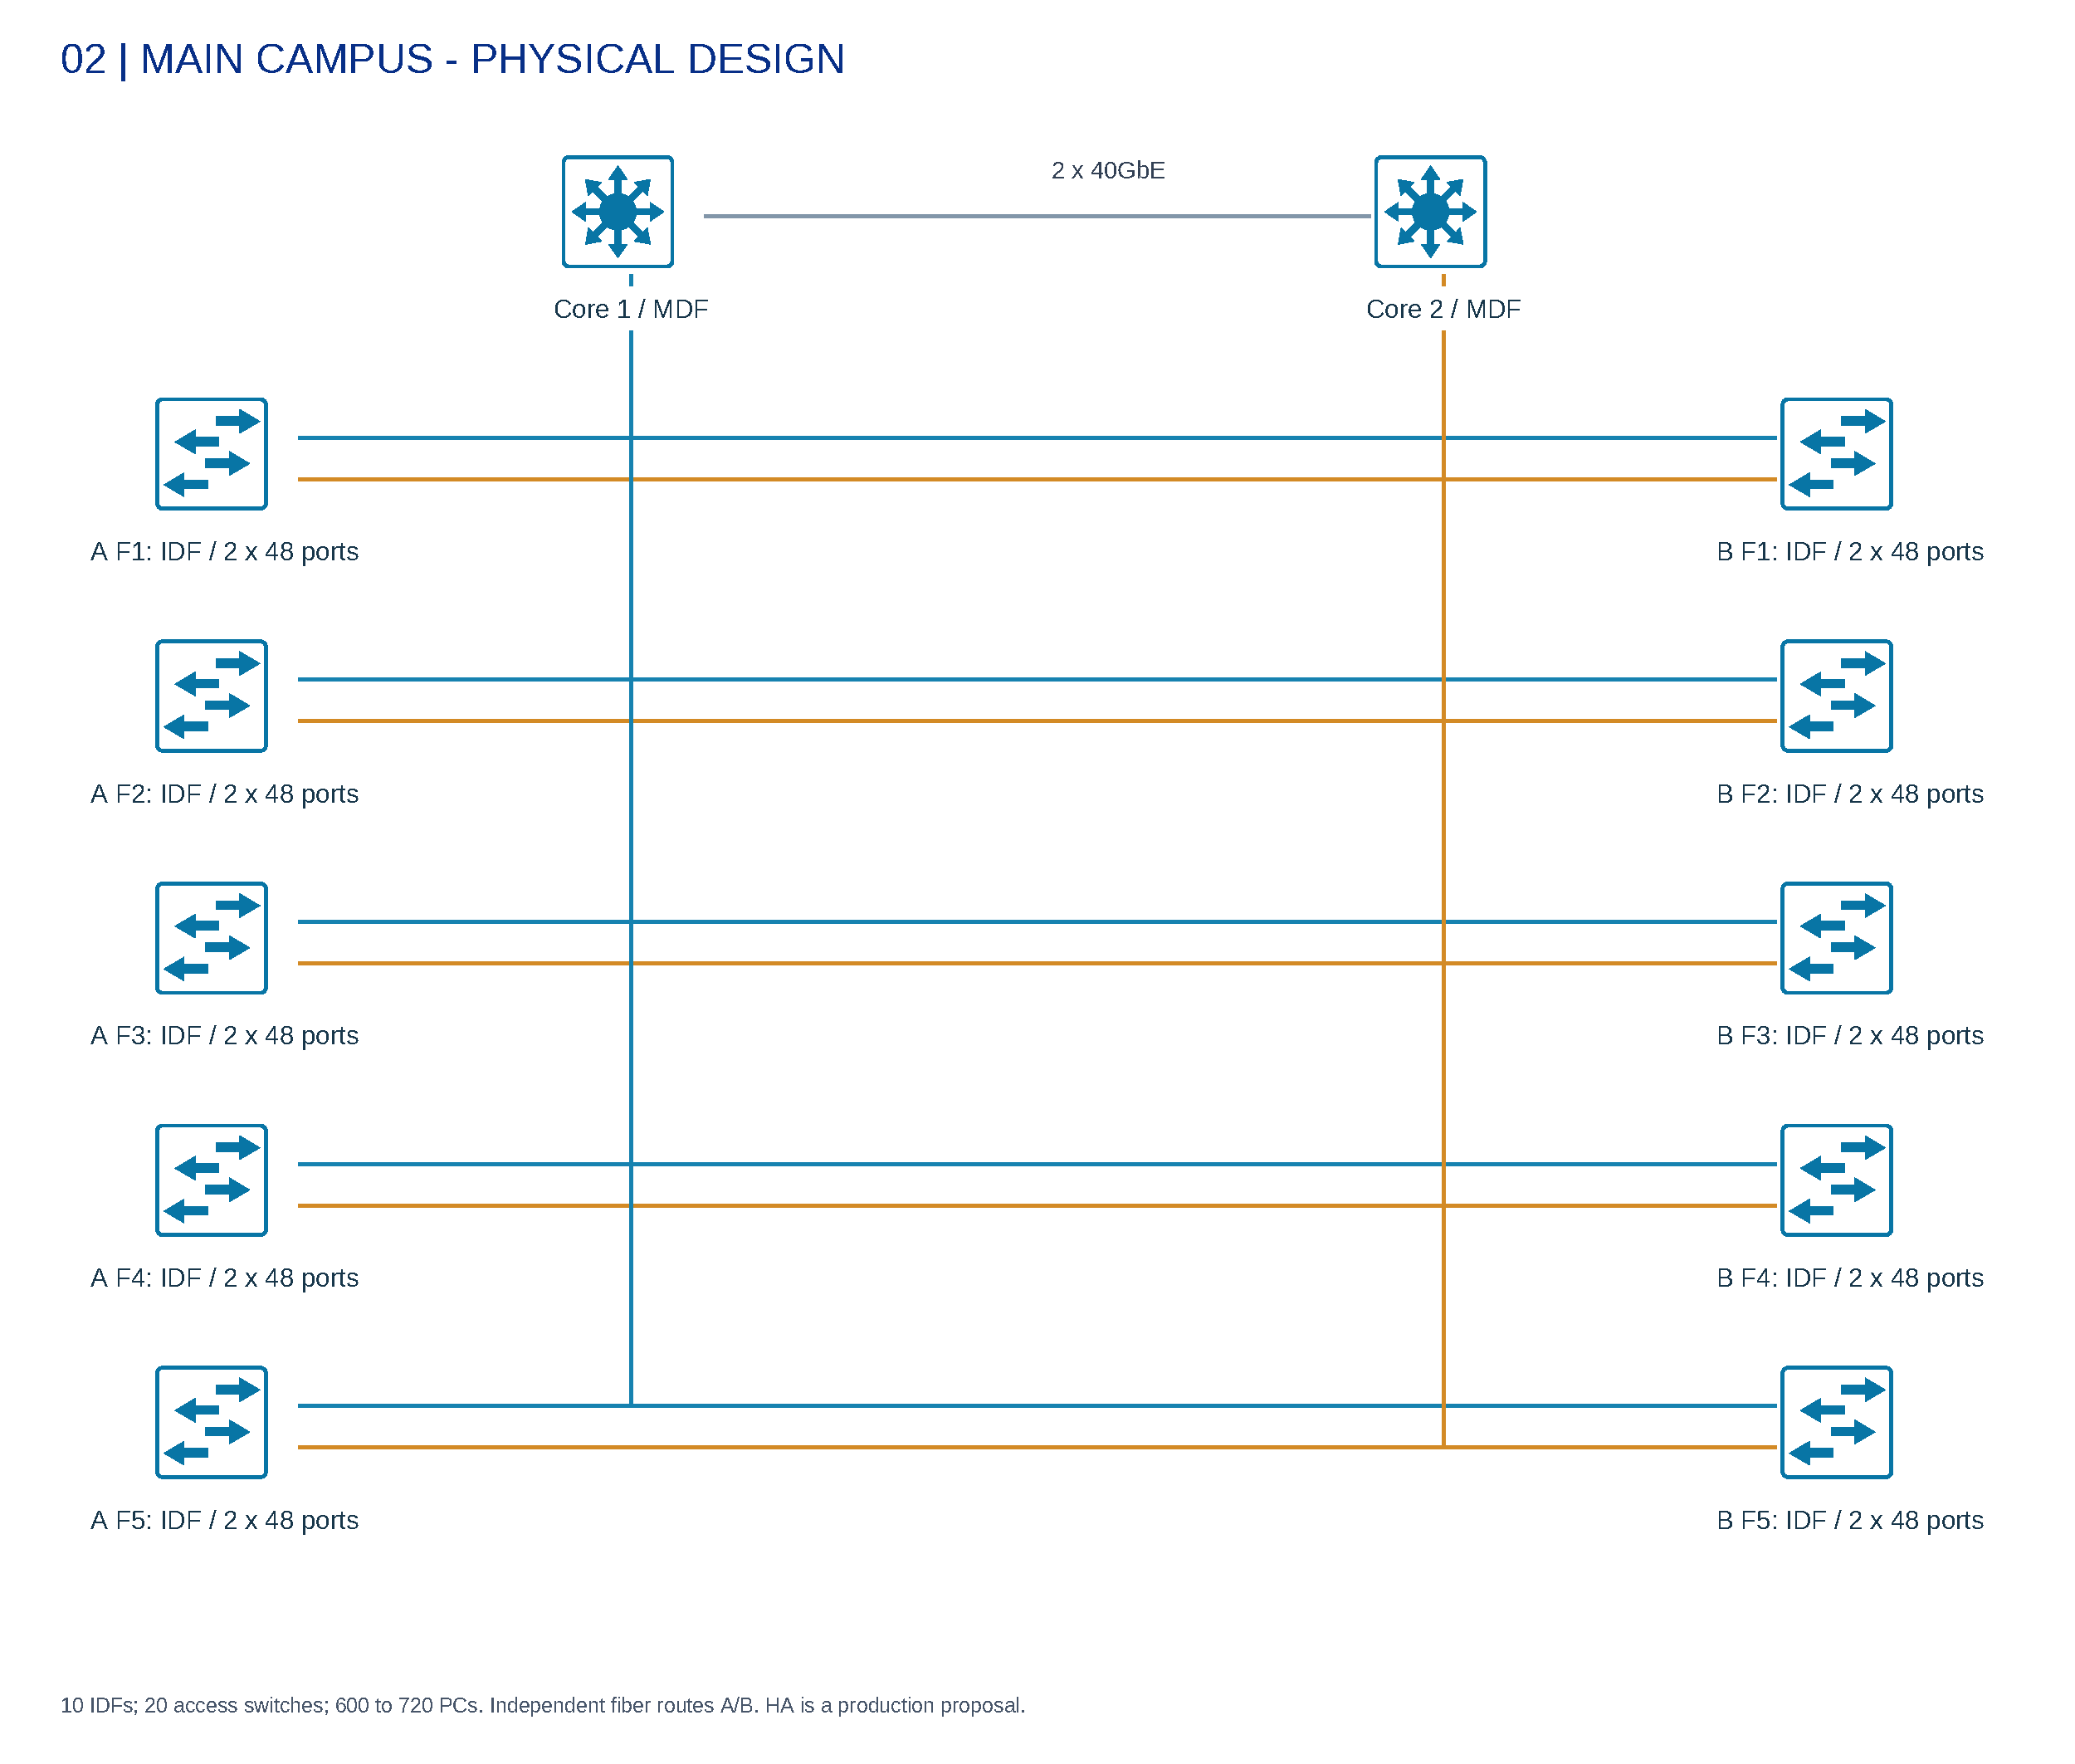
\includegraphics[width=.49\linewidth,height=.35\textheight,keepaspectratio]{assets/main-cisco.pdf}\hfill
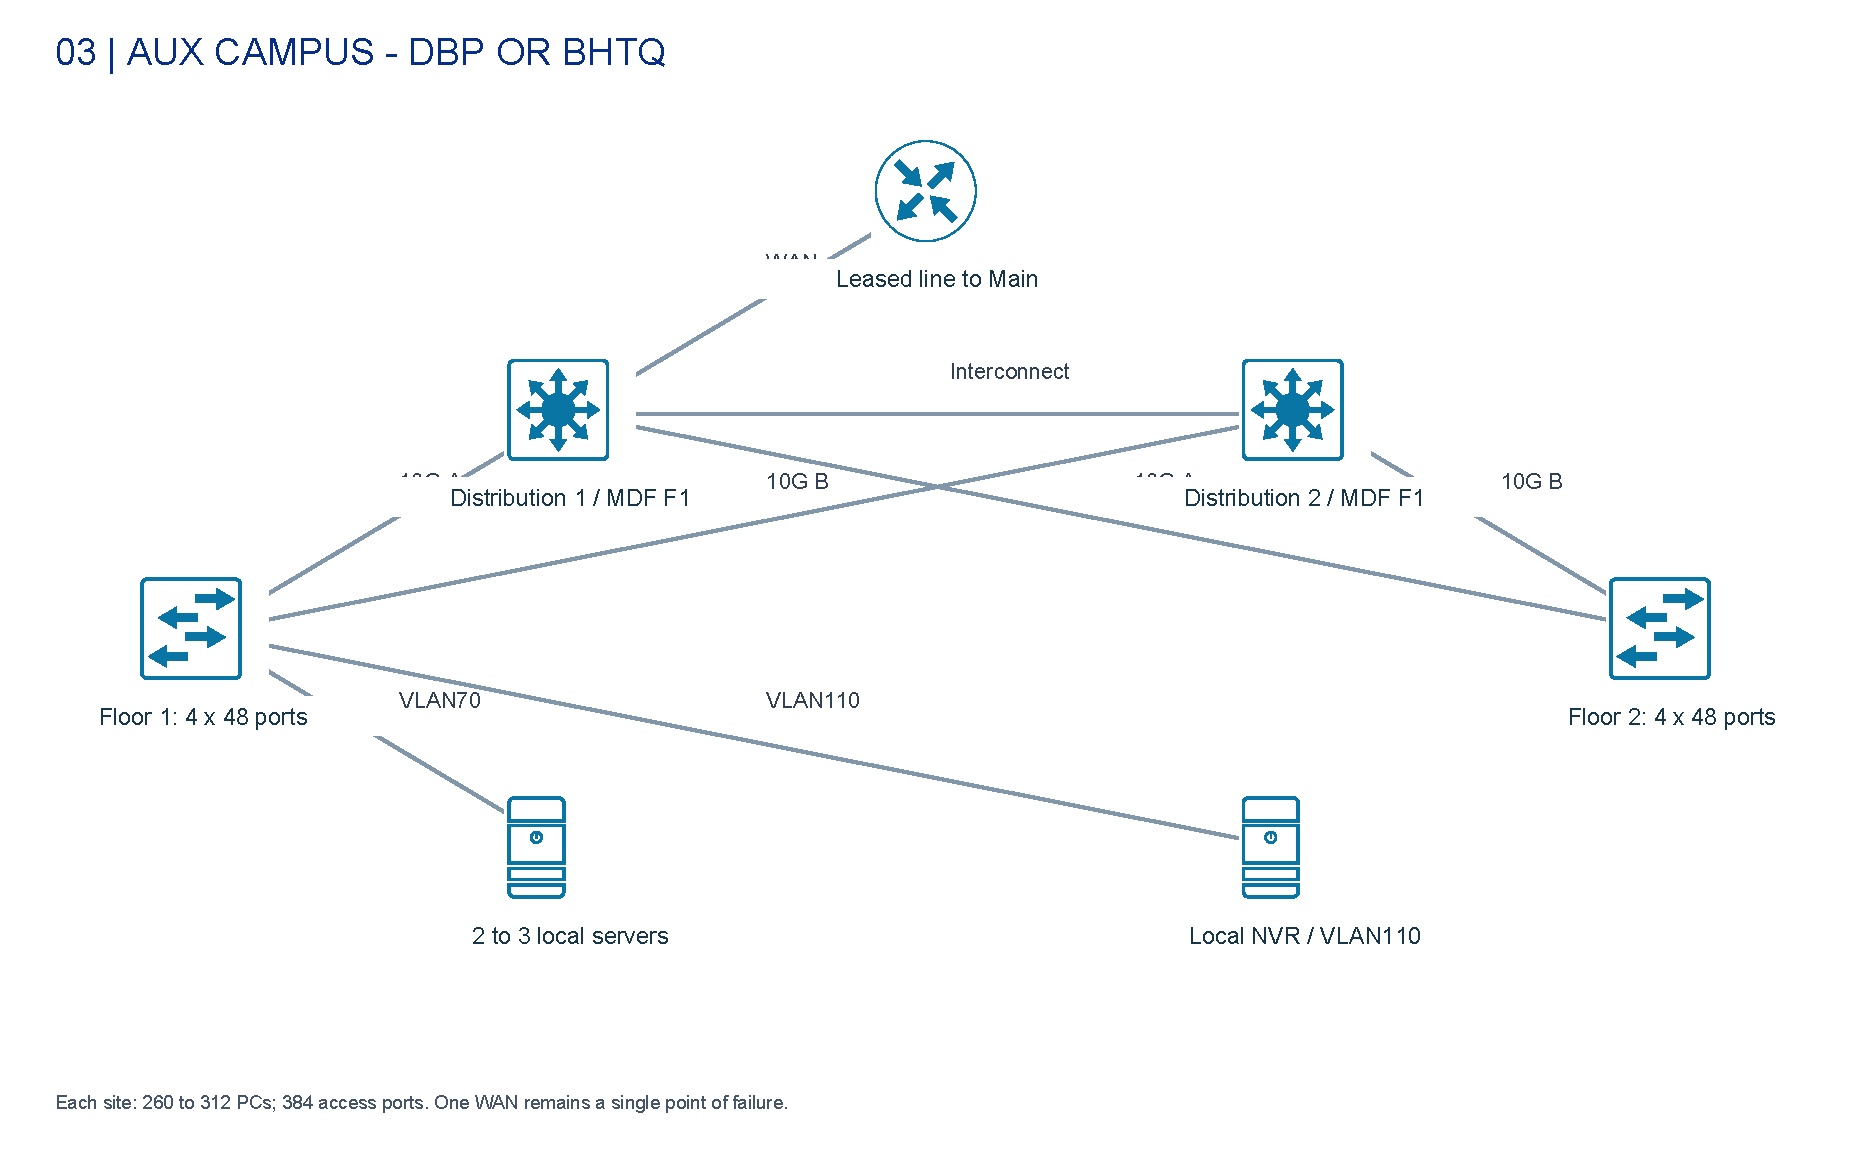
\includegraphics[width=.49\linewidth,height=.35\textheight,keepaspectratio]{assets/aux-cisco.pdf}
\captionof{figure}{Mặt bằng Main và Aux với các tuyến uplink quang.}
\end{center}
\par\noindent
\tabletitle{Số lượng uplink và tuyến cáp quang campus}
\begin{tabularx}{\linewidth}{@{}lXX@{}}\toprule
Hạng mục & Main & Mỗi Aux\\\midrule
Access uplink 10 G & 40 link duplex & 16 link duplex\\
Lý do & 20 switch, 2 uplink/switch & 8 switch, 2 uplink/switch\\
Tuyến đứng điển hình & 2 switch/IDF: 8 sợi tổng, chia 4/tuyến & Tầng 2: 8 link duplex, 8 sợi/tuyến\\
Cáp dự trù & OS2, tuyến A/B và ODF riêng & Hai cáp 12 sợi cho tầng 2\\\bottomrule\end{tabularx}\par

Toàn bộ campus có 72 link uplink quang. SFP cần hai đầu/link: 144 module cho access uplink, chưa gộp core/server/WAN. Tên cổng Te trong kế hoạch phải remap theo thiết bị được mua.

Giới hạn channel đồng kiểm theo tiêu chuẩn/cáp thực tế. Cổng FastEthernet của 2960-24TT trong Packet Tracer chỉ 100 Mbps; ảnh lab không nghiệm thu 1/10/40 GbE sản xuất. LACP vào cùng một core trong lab cũng không tạo HA hai chassis.

\clearpage
\subsection{VLAN và địa chỉ ba cơ sở}
Khối site: Main 10.10/16, DBP 10.20/16, BHTQ 10.30/16. Đặt $S=10,20,30$ tương ứng. Gateway thông thường \texttt{10.S.VLAN.1}; VLAN cùng mã giữa các site vẫn là các subnet riêng.
\par\noindent
\tabletitle{Phân chia VLAN và địa chỉ IP}
\begin{tabularx}{\linewidth}{@{}lXXX@{}}\toprule
VLAN / vai trò & Main & Mỗi Aux & Cấp phát\\\midrule
10,20,30 / nghiệp vụ & 10.10.V.0/25 & 10.S.V.0/25 & .7--.126\\
40,50,60 / nghiệp vụ & 10.10.V.0/25 & Không dùng trong lab & .7--.126\\
70 / Server Farm & 10.10.70.0/27 & 10.S.70.0/28 & Tĩnh\\
80 / DMZ & 10.10.80.0/27 & Không có & Tĩnh, GW trên FW\\
90 / quản trị & 10.10.90.0/24 & 10.S.90.0/24 & Tĩnh\\
100 / Guest & 10.10.100.0/23 & 10.S.100.0/23 & .100.11--.101.254\\
110 / camera & 10.10.110.0/24 & 10.S.110.0/24 & Tĩnh\\
120 / Staff & 10.10.120.0/24 & 10.S.120.0/24 & .11--.254\\\bottomrule\end{tabularx}\par

Mỗi /25 có 126 địa chỉ usable; chừa .1 gateway và .2--.6 hạ tầng, còn đúng 120 lease. Main mỗi VLAN PC có 100 máy lên 120; Aux 90/90/80 lên 108/108/96. Main vì vậy hết dư pool nghiệp vụ ở năm thứ 5; nếu tăng hơn cần tách VLAN hoặc mở subnet/pool có kế hoạch.

Guest /23 cho 500 lease; Staff /24 cho 244 lease. Số lease không thay được tính số thiết bị đồng thời và airtime. Các subnet quản trị/camera được quy hoạch nhưng không phải mọi endpoint production đều đã có trong lab.

Dải transit gồm 10.255.0.0/30 và các /30 tiếp theo theo bảng IP đầy đủ. ISP dùng TEST-NET 203.0.113/24, 198.51.100/24; Web-Lab 192.0.2.100. Đây là địa chỉ mô phỏng, không phải public IP đã được nhà mạng cấp.

\clearpage
\subsection{Server Farm, DMZ, DHCP và DNS}
\par\noindent
\tabletitle{Phân bố máy chủ và vai trò dịch vụ}
\begin{tabularx}{\linewidth}{@{}lXX@{}}\toprule
Site / vùng & Địa chỉ & Chức năng\\\midrule
Main VLAN 70 & 10.10.70.10--17 & DNS/Infra, HIS, PACS, LIS, CRM, DB, Backup, Monitor\\
Main VLAN 80 & 10.10.80.10--11 & Web DMZ và Proxy, tách sau firewall\\
DBP VLAN 70 & 10.20.70.6--7 & Infra/DNS và server cục bộ\\
BHTQ VLAN 70 & 10.30.70.6--7 & Infra/DNS và server cục bộ\\
Ngoài bệnh viện & 192.0.2.100 & Web-Lab và DNS công cộng mô phỏng\\\bottomrule\end{tabularx}\par

14 server bệnh viện gồm 10 Main và 2 tại mỗi Aux; Web-Lab là server thứ 15 ngoài phạm vi đó. Ba Server-PT IoT .110.12 thuộc VLAN110, ngoài 14 server ứng dụng; ba PC-PT tên NVR .110.11 chỉ đại diện thiết kế lưu video. Tên HIS/PACS/DB biểu diễn vai trò; HTTP marker trong lab không phải phần mềm bệnh viện đã triển khai.

Dịch vụ DHCP/DNS được mô hình hóa bằng Server-PT \cite{pt-servers}. DHCP có 8 pool Main và 5 pool mỗi Aux, tổng 18 pool cấp phát. Ba pool mặc định \texttt{serverPool} đặt capacity 0 để không cấp sai subnet; vẫn tồn tại trong saved state. VLAN server, DMZ và quản trị dùng IP tĩnh. Relay gateway chuyển DHCP tới server đúng site.

DNS nội bộ Main 10.10.70.10, Aux .70.6. Các bản ghi gồm \texttt{his.hospital.test} $\to$ 10.10.70.11, tên PACS/LIS/CRM tương ứng và \texttt{web.hospital.test} $\to$ 192.0.2.100. Guest dùng DNS ngoài lab, không phải được mở quyền vào DNS nội bộ chỉ để chạy test.

Static PAT công bố TCP 198.51.100.2:8080 về 10.10.80.10:80; firewall chỉ mở dịch vụ đã duyệt. Phải kiểm HTTP từ ngoài, nội dung đúng, translation và chiều trả lời. Ping thành công không chứng minh publish Web đúng.

Triển khai thực tế cần TLS, tài khoản, backup/restore và giám sát ứng dụng riêng.

\clearpage
\subsection{Cáp quang và GPON hybrid}
Chọn GPON cho 80/100 PC hành chính VLAN 60 ở Main, 20 PC còn lại dùng Ethernet. Sau tăng trưởng tương ứng 96/24, tổng 120 PC. Các VLAN nghiệp vụ, AP, camera và server giữ Ethernet để giới hạn miền lỗi và độ phức tạp.
\pic{assets/gpon-cisco.pdf}{.35\textheight}{Đề xuất GPON chỉ cho nhánh hành chính; không phải kết quả PHY đã đo.}

2 PON port, mỗi port splitter 1:16; 20 ONT hiện tại lên 24 ONT, 4 GE user port/ONT cho 80 lên 96 PC. Một OLT vẫn là SPOF; chưa có bảo vệ Type B/C. Uplink OLT chỉ cho VLAN 60 và quản trị 90, không bridge DMZ/Guest/Server Farm vào ODN.

Ngân sách suy hao giả định: 0,5 km sợi $\times$ 0,35 dB/km, splitter 13,5 dB, 4 connector $\times$ 0,5 dB, 4 mối hàn $\times$ 0,1 dB:
\[L_{ODN}=0,175+13,5+2+0,4=16,075\ \mathrm{dB}.\]
Thêm dự phòng 3 dB được 19,075 dB; so cửa sổ class B+ 13--28 dB \cite{g984} còn 8,925 dB ở đầu suy hao cao. Phải kiểm cả overload tuyến ngắn, Tx/Rx theo model, đo OTDR/power và vệ sinh connector.

GPON chia sẻ 2,488/1,244 Gbps danh nghĩa; 4 GE/ONT không có nghĩa mọi cổng đạt đồng thời line rate. DBA, OMCI, GEM/T-CONT và VLAN translation cần kiểm thiết bị thật.

\clearpage
\subsection{Wi-Fi Staff và Guest}
\pic{assets/wifi-cisco.pdf}{.35\textheight}{Phân SSID/VLAN và quản trị AP trong phương án triển khai.}
Dự trù Main 30 AP, mỗi Aux 6 AP; sau 5 năm 40/8/8. Đây là ngân sách ban đầu theo tầng, chưa có khảo sát RF. Nghiệm thu phải kiểm RSSI/SNR, nhiễu, airtime, roaming, số phiên và throughput trong điều kiện tải.

\par\noindent
\tabletitle{Ánh xạ mạng không dây và quyền truy cập}
\begin{tabularx}{\linewidth}{@{}lXX@{}}\toprule
Mạng & Ánh xạ & Quyền\\\midrule
Staff & VLAN 120 & Dịch vụ nội bộ được duyệt và Internet\\
Guest & VLAN 100 & DHCP/DNS và Web Internet, chặn nội bộ\\
Quản trị AP & VLAN 90 & Máy quản trị có quyền\\\bottomrule\end{tabularx}\par

Packet Tracer giữ 6 AP cũ, bổ sung 8 AP tầng dùng SSID riêng; cả 14 nối access VLAN. Sáu client card PT-HOST-NM-1W-AC được kiểm association riêng. Native kiểm WPA2-PSK, BSSID, IP/lease và truy cập; không chứng minh WLC, WPA3, 802.1X/RADIUS hoặc roaming production.

Thiết kế thực đề xuất WPA2/WPA3-Enterprise theo khả năng model và RADIUS; không gọi WAP54G là AP dual-band/WPA3. Datasheet Linksys WAP54G-EU V1 \cite{wap54g} mô tả 802.11b/g, 54 Mbps và WPA/WEP; không có cơ sở cho tuyên bố WPA3. Bản tham khảo có cách trình bày SSID rõ nhưng phải kiểm đúng thiết bị/version.

Khóa lab công khai chỉ phục vụ mô phỏng, cần thay khi triển khai.

\clearpage
\subsection{Camera, NVR và lưu trữ}
Đặc tả yêu cầu đề xuất hệ thống camera; không ấn định số camera, thời gian lưu hoặc demo ghi hình. Thiết kế giả định 4 camera/tầng, tăng thành 5/tầng; bitrate 4 Mbps/camera, giữ 30 ngày. Cần khảo sát góc nhìn, vùng riêng tư và bitrate thực trước triển khai.
\par\noindent
\tabletitle{Quy mô camera và dung lượng lưu trữ đề xuất}
\begin{tabularx}{\linewidth}{@{}lXXX@{}}\toprule
Thông số & Main & DBP & BHTQ\\\midrule
Camera nay / 5 năm & 40 / 50 & 8 / 10 & 8 / 10\\
Video Mbps nay / 5 năm & 160 / 200 & 32 / 40 & 32 / 40\\
Raw 30 ngày hiện tại & 51.840 GB & 10.368 GB & 10.368 GB\\
Usable cần nay & 68.040 GB & 13.608 GB & 13.608 GB\\
Usable cần sau 5 năm & 85.050 GB & 17.010 GB & 17.010 GB\\\bottomrule\end{tabularx}\par
\[Raw_{GB}=\frac{N\,b\,10^6\times86400\times30}{8\times10^9},\quad
Usable_{GB}=Raw_{GB}\frac{1,05}{0,80}.\]
5\% overhead ghi và giới hạn sử dụng 80\% sau RAID là giả định riêng, không thay bằng tăng trưởng 20\%. Ví dụ Main 12 ổ 10 TB RAID6 có 100 TB lý thuyết trước filesystem; Aux 4 ổ 12 TB RAID6 có 24 TB. Cần kiểm usable thật, rebuild, hot spare, kênh/ingest và ổ được NVR hỗ trợ. RAID không thay backup.

VLAN 110 dùng IP tĩnh, NVR .110.11; ghi cục bộ không đi WAN. Chỉ quản trị có quyền xem, không port-forward NVR ra Internet. Cùng VLAN trao đổi L2 nên ACL gateway không bảo vệ mọi luồng camera--NVR; phải có quyền ứng dụng và bảo vệ endpoint.

File \texttt{hospital-3sites.pkt} có 14 webcam đại diện: Main 10, DBP 2, BHTQ 2; mỗi tầng một mẫu, không thay số lượng thiết kế trong bảng. Ba server IoT .110.12 quản lý đăng ký/trạng thái; ba PC-PT tên NVR .110.11 chỉ đại diện vị trí lưu video, chưa thực thi ghi hình. Kết quả kiểm thử được trình bày ở mục \ref{sec:camera-tests}.

\clearpage
\subsection{WAN, OSPF và chi phí phương án}
\pic{assets/wan-cisco.pdf}{.30\textheight}{Hai nhánh leased line về Main và Internet tập trung qua hai ISP.}
Baseline hai leased line routed, OSPF area 0 giữa Main-Core, Main-GW và Aux-GW. Mạng user đặt passive; Firewall/Edge dùng route tĩnh kiểm soát. Mỗi Aux một WAN vẫn là SPOF. MPLS/SD-WAN là phương án so sánh, không gọi OSPF/PBR là SD-WAN.
\par\noindent
\tabletitle{So sánh phương án WAN và TCO minh họa}
\begin{tabularx}{\linewidth}{@{}lXX@{}}\toprule
Phương án & Giá trị / điều kiện & TCO 5 năm minh họa\\\midrule
Metro-E/leased & Bám hai tuyến, OSPF; chốt SLA/handoff & 1.745 triệu VNĐ\\
MPLS L3VPN & VRF provider, ba CE; không tự mã hóa & 1.948 triệu VNĐ\\
SD-WAN + leased & Controller, license, chính sách ứng dụng & 2.105 triệu VNĐ\\
IPsec + leased & Crypto/MTU/CPU và khóa cần nghiệm thu & 1.775 triệu VNĐ\\\bottomrule\end{tabularx}\par

\textbf{Tất cả số tiền là giả định tính TCO}, chưa có báo giá/VAT/SLA cùng phạm vi. Công thức $CAPEX+60\times OPEX_{\text{tháng}}+\text{bảo trì}$. Ví dụ Metro-E: $155+60\times25,5+60=1745$ triệu. Không dùng bảng này để khẳng định nhà mạng rẻ nhất; tránh cộng trùng CPE/quang/BOM.

Đề yêu cầu hai xDSL load balancing. Lab thay đường đồng bằng Ethernet chức năng, chưa đo DSL. Nếu xDSL không đáp ứng tải hai chiều, quang doanh nghiệp/DIA là đề xuất thay thế cần chấp thuận khi triển khai.

\clearpage
\subsection{Chính sách vùng và hai phương án VPN}
\begin{center}
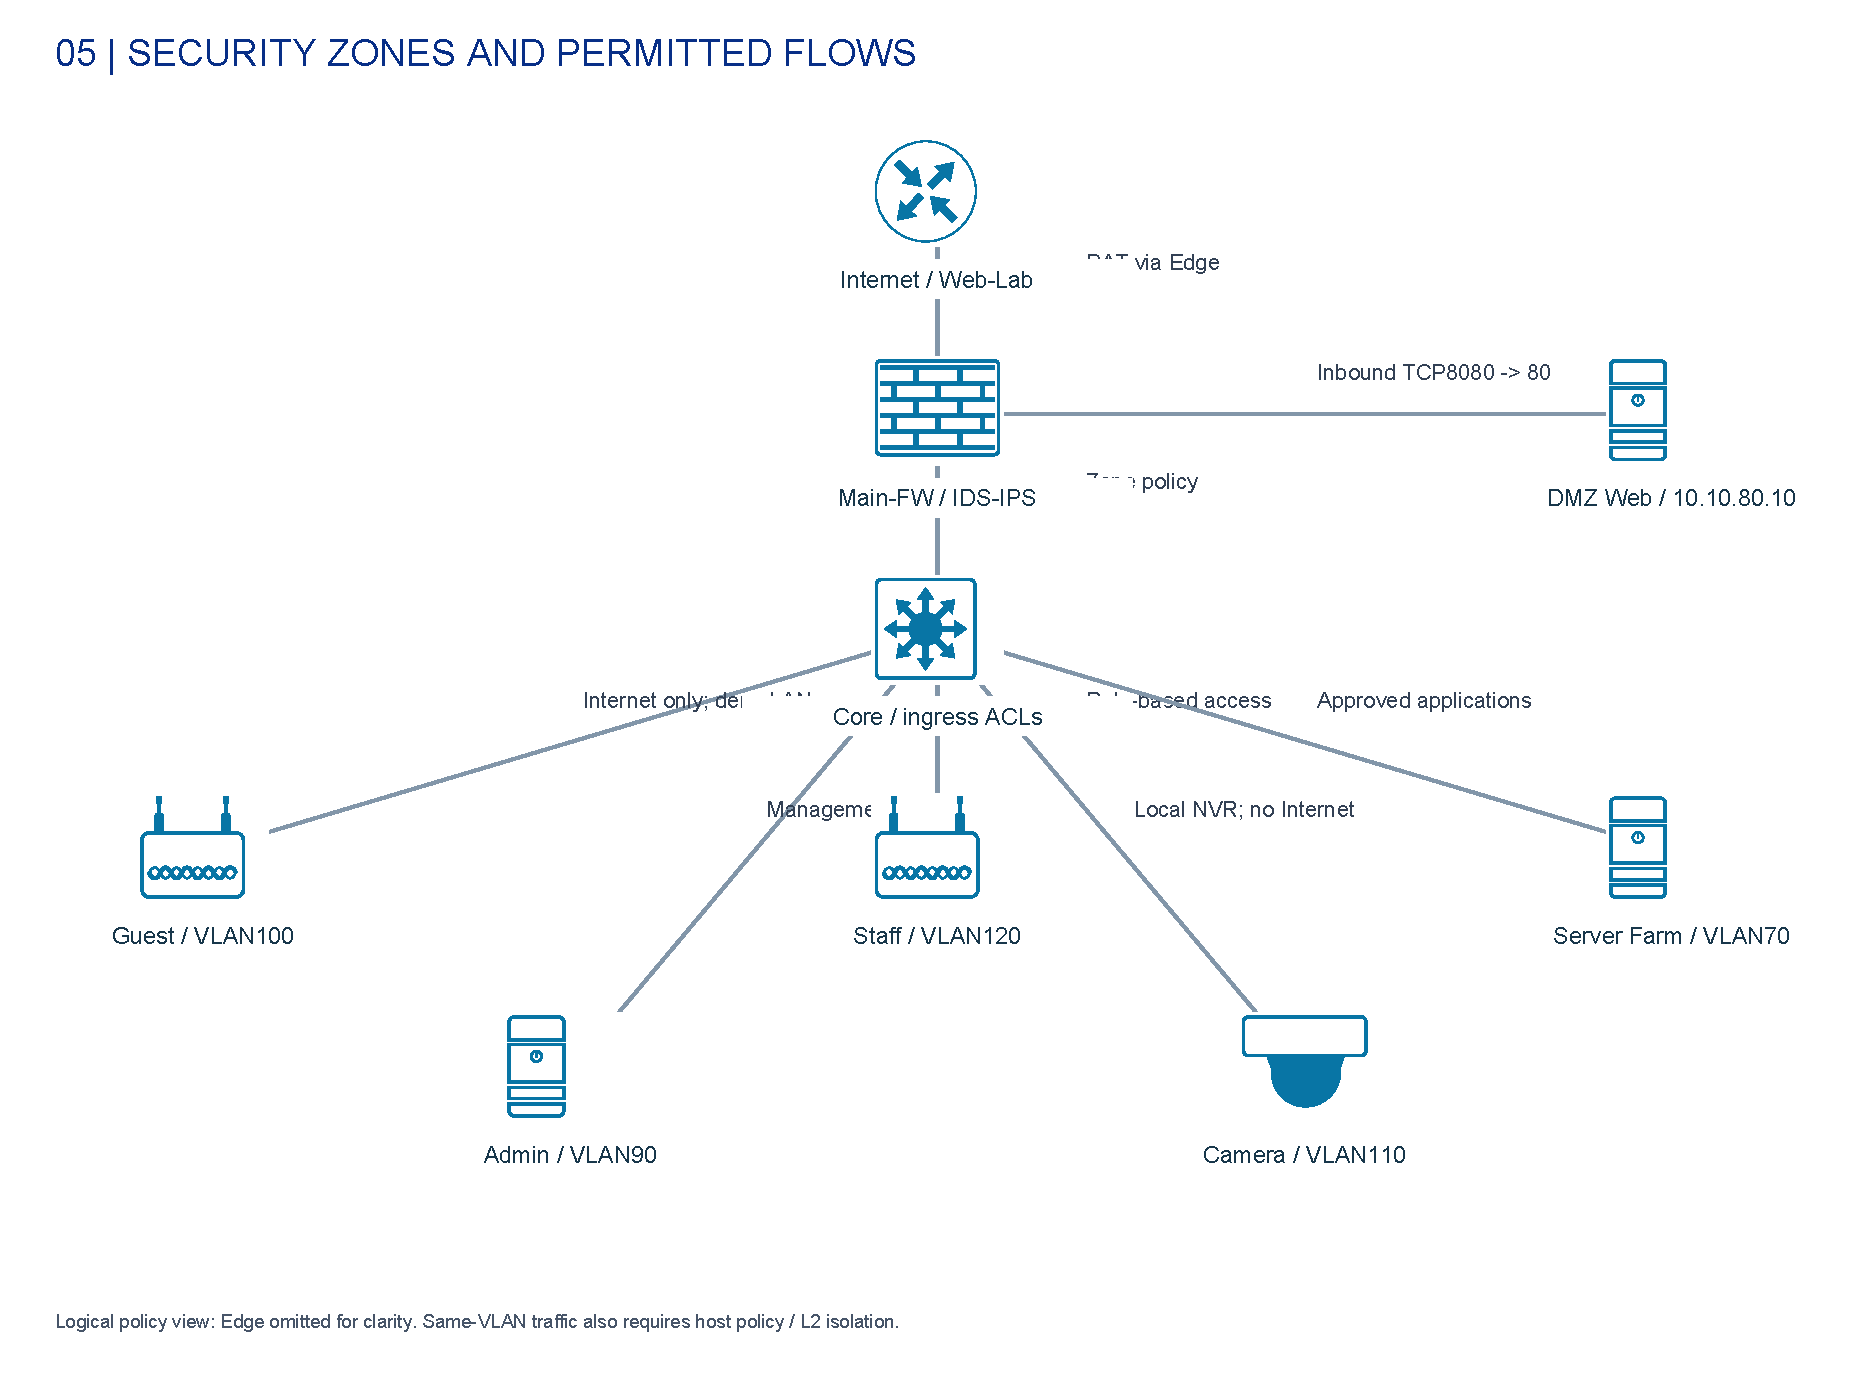
\includegraphics[width=.49\linewidth,height=.30\textheight,keepaspectratio]{assets/security-cisco.pdf}\hfill
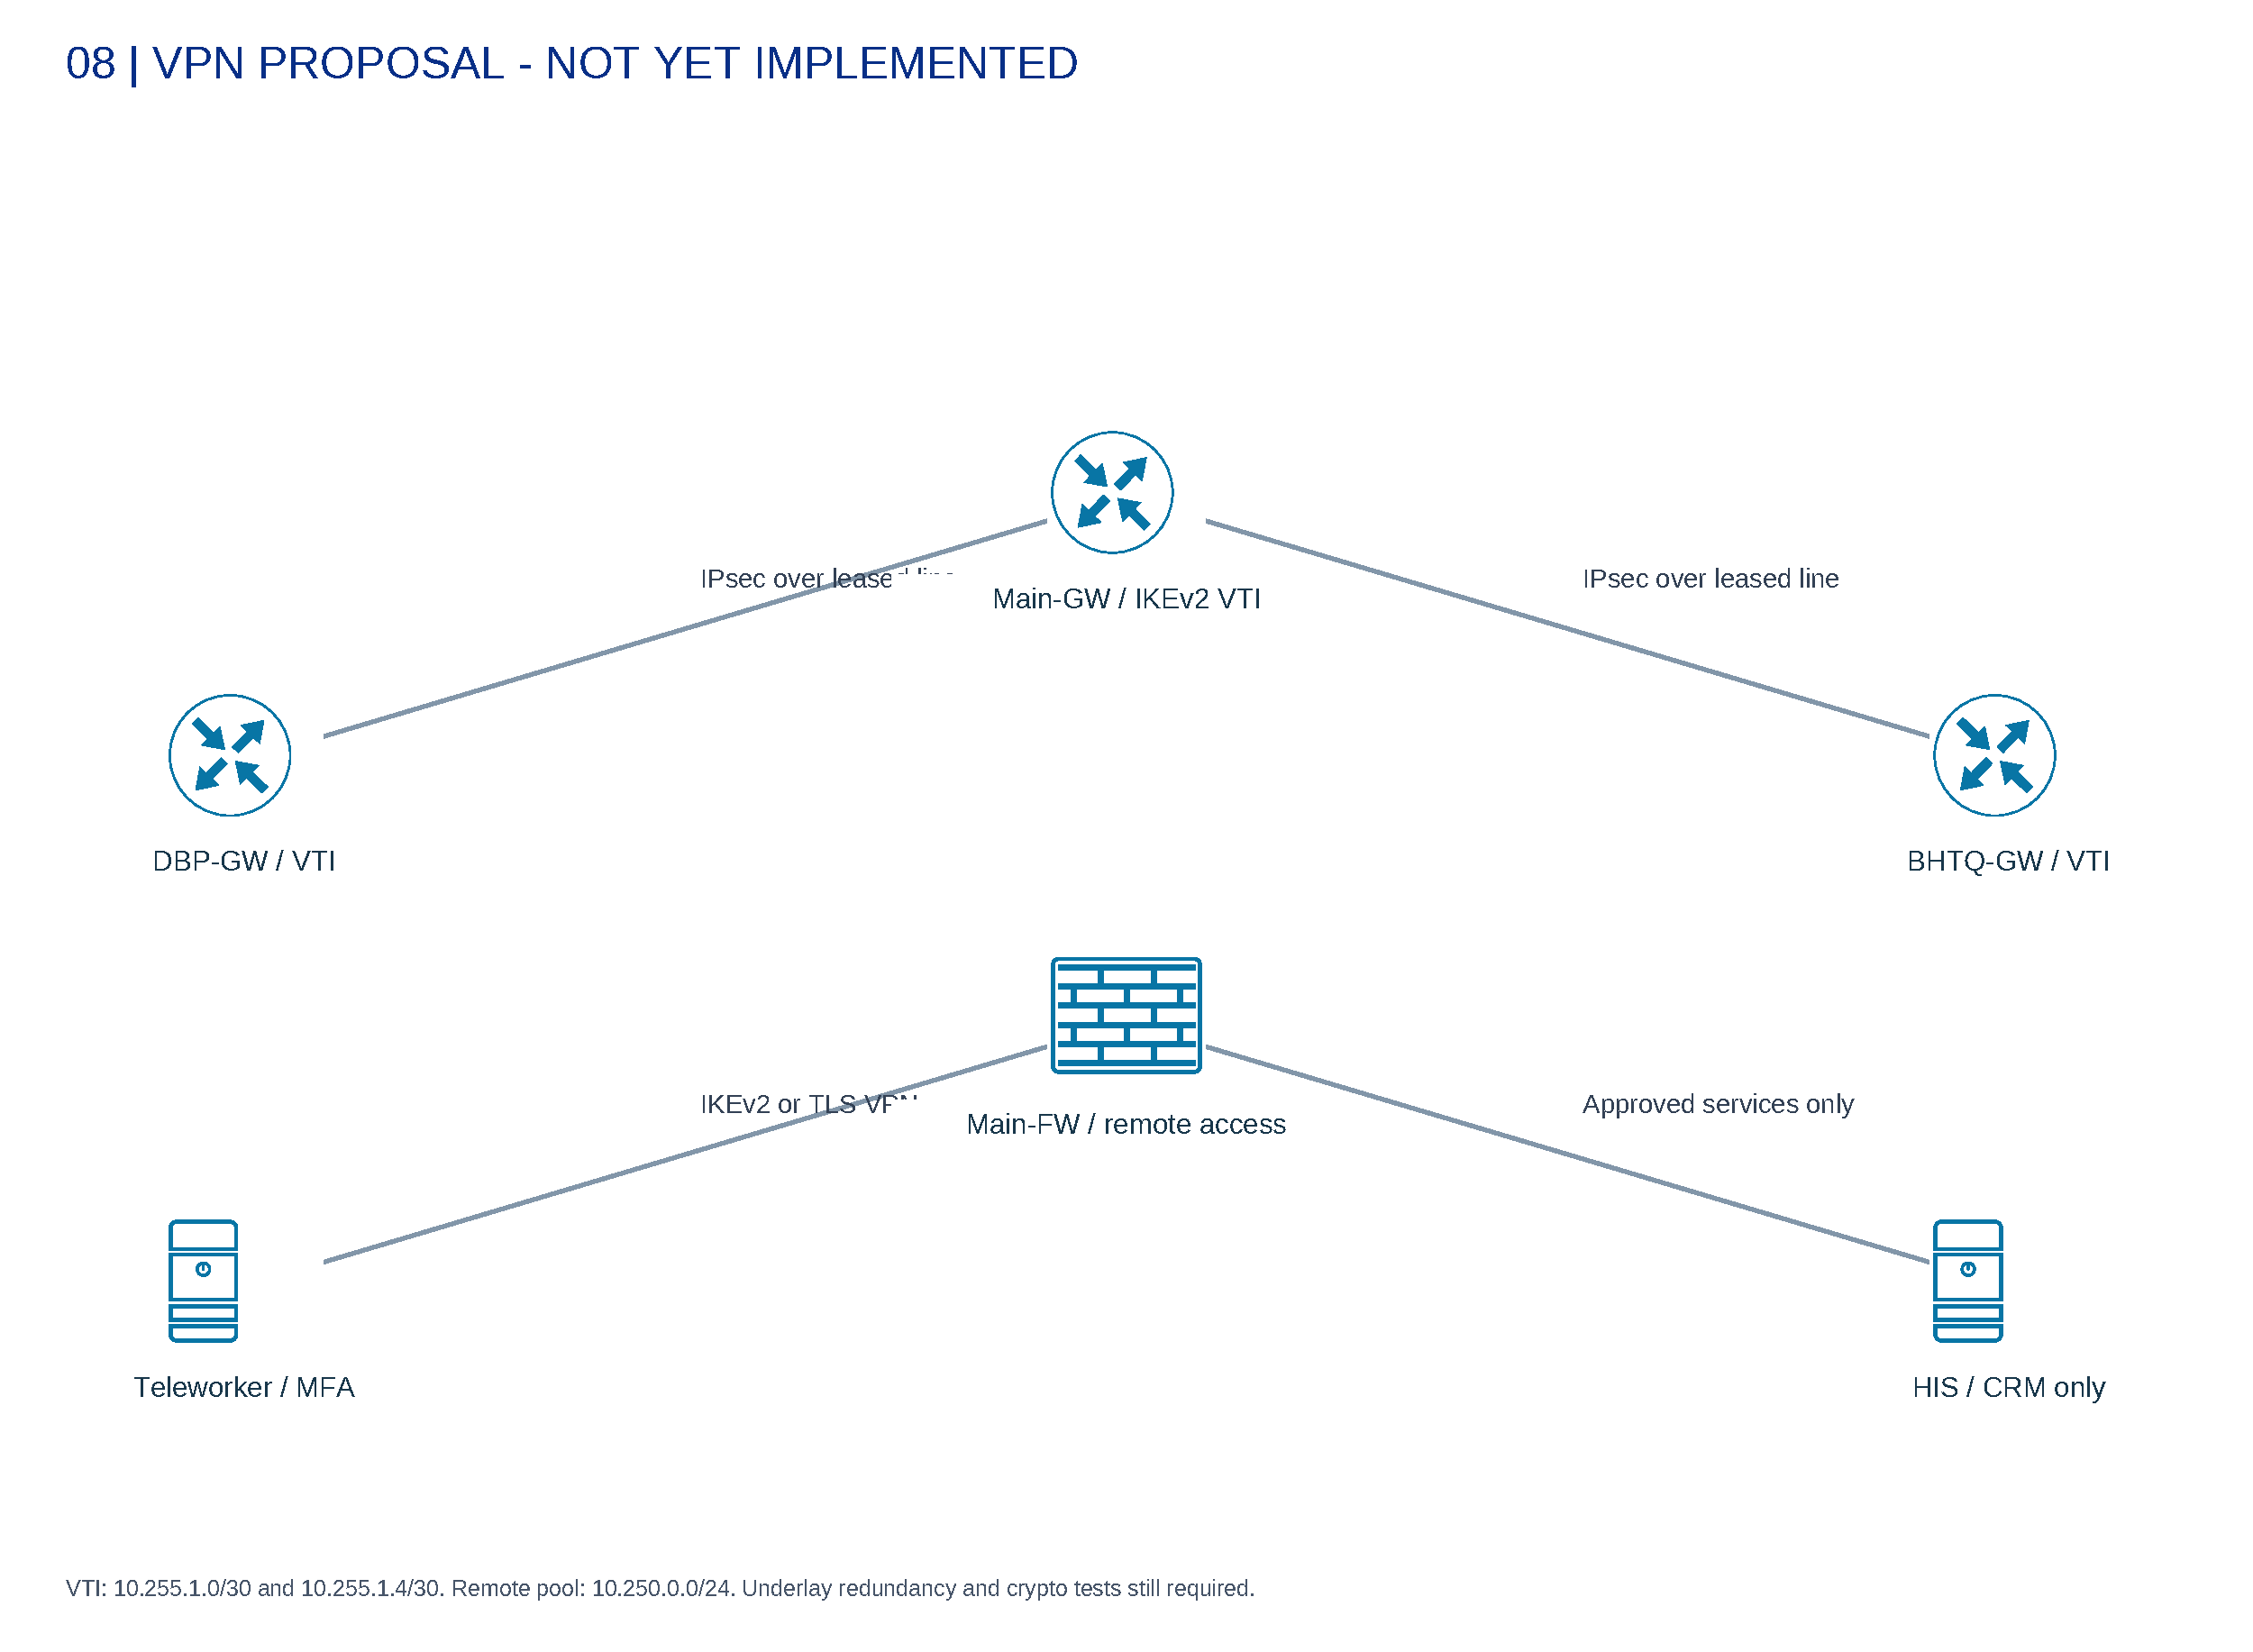
\includegraphics[width=.49\linewidth,height=.30\textheight,keepaspectratio]{assets/vpn-cisco.pdf}
\captionof{figure}{Phân vùng bảo mật và hai phương án VPN đề xuất.}
\end{center}
\par\noindent
\tabletitle{Chính sách truy cập giữa các vùng}
\begin{tabularx}{\linewidth}{@{}lXX@{}}\toprule
Nguồn & Đích & Chính sách\\\midrule
PC nghiệp vụ / Staff & HIS và dịch vụ được duyệt & Cho phép theo vai trò\\
Guest & LAN, Farm, quản trị, camera & Chặn; giữ DHCP/DNS/Web ngoài\\
Internet & DMZ Web & Chỉ cổng publish đã duyệt\\
Internet / user thường & Camera, quản trị & Không mở quyền mặc định\\
Main-Admin & Thiết bị / NVR & Quản trị riêng, tài khoản tối thiểu\\\bottomrule\end{tabularx}\par

\textbf{Site-to-site VPN đề xuất:} route-based IPsec Main--Aux, IKEv2, chính sách prefix rõ ràng; thiết kế NAT exemption, route chiều trả lời, MTU/MSS và quản lý khóa/chứng thư. Không NAT Internet cho giao dịch private liên site.

\textbf{Teleworker VPN đề xuất:} kết thúc tại firewall/VPN gateway Main, pool riêng 10.250.0.0/24, MFA, chỉ cấp quyền ứng dụng đã duyệt. Chốt split/full tunnel, DNS, logging, thời hạn phiên và thu hồi tài khoản.

Hai VPN chưa triển khai runtime; không có SA/crypto/teleworker log để gán PASS. MPLS L3VPN phân tách route không thay mã hóa IPsec. ACL liên VLAN không thay host firewall và quyền HIS/DB, đặc biệt khi hai máy cùng VLAN.

ACL, ZBF và NAT đã có kiểm chức năng Cisco; IDS/IPS và chống phishing vẫn là phương án thiết kế, chưa có cảnh báo/drop native để nghiệm thu.

\clearpage
\section{Tính tải và băng thông (Step 3)}
\subsection{Đầu vào, đơn vị và giả định}
\par\noindent
\tabletitle{Đầu vào và giả định tính băng thông}
\begin{tabularx}{\linewidth}{@{}lXX@{}}\toprule
Đầu vào & Download & Upload\\\midrule
Mỗi workstation & 500 MB/ngày & 100 MB/ngày\\
Server (cách hiểu bảo thủ mỗi máy) & 1.000 MB/ngày & 2.000 MB/ngày\\
Mỗi thiết bị khách/ngày (giả định) & 500 MB/ngày & Chưa được cho\\
Cửa sổ cao điểm & 80\% dung lượng trong 3 giờ & 09--11 và 15--16\\
Tăng trưởng / sử dụng & Tổng 20\% trong 5 năm & $U=70\%$ giả định\\\bottomrule\end{tabularx}\par

MB thập phân $=10^6$ byte, một byte 8 bit. Với $D$ là MB/ngày, $P=0,8$, $T=10800$ s, $g=0,2$:
\[B_{peak}=\frac{D\times8\times P}{T}\ (Mbps),\qquad
B_{design}=\frac{B_{peak}(1+g)}{U}.\]
Hệ số sử dụng 70\% tạo dư địa thiết kế: đường được chọn cao hơn tải trung bình cửa sổ cao điểm. Đây không phải mức sử dụng đo được hoặc một yêu cầu đề bài. $B_{peak}$ chưa phải đỉnh tức thời; overhead và tải y tế chuyên biệt chưa định lượng.

Đặc tả dùng chữ ``total'' cho server, có thể hiểu tổng toàn viện/từng site. Báo cáo giữ kịch bản mỗi server làm envelope bảo thủ và nêu cả cách hiểu tổng, thay vì coi giả định là dữ kiện. Số khách chưa được cung cấp: dùng biến $N_M,N_D,N_B$, phân biệt số theo ngày với số đồng thời.

Chưa có dữ liệu upload khách; phần upload tính được là tải đã biết. Camera/PACS/backup chỉ cộng phần chưa nằm trong định mức sau khảo sát để tránh đếm đôi.

\clearpage
\subsection{Kết quả kiểm được theo cơ sở}
Kịch bản mỗi server, chưa có khách:
\[D_{down}=1120\times500+14\times1000=574000,\]
\[D_{up}=1120\times100+14\times2000=140000\ \mathrm{MB/ngày}.\]
\par\noindent
\tabletitle{Kết quả tính tải theo cơ sở}
\begin{tabularx}{\linewidth}{@{}lXXX@{}}\toprule
Site & MB/ngày down / up & Peak Mbps down / up & Design Mbps down / up\\\midrule
Main & 310.000 / 80.000 & 183,70 / 47,41 & 314,92 / 81,27\\
DBP & 132.000 / 30.000 & 78,22 / 17,78 & 134,10 / 30,48\\
BHTQ & 132.000 / 30.000 & 78,22 / 17,78 & 134,10 / 30,48\\
Toàn viện & 574.000 / 140.000 & 340,15 / 82,96 & 583,11 / 142,22\\\bottomrule\end{tabularx}\par

Ví dụ Main down: $310000\times6,4/10800=183,7037$ Mbps; nhân $1,2/0,7$ được 314,9206 Mbps. Làm tròn để trình bày, calculator giữ độ chính xác đầy đủ trong CSV. Không cộng down và up để chọn tốc độ một chiều của đường full duplex.

\textbf{Ranh giới tải.} PC Main tới HIS local không đi ISP. PC Aux tới HIS đi leased line nhưng không ra Internet. Giao dịch tới dịch vụ công/y văn/email ngoài mới đi Main Internet Edge. Con số 583,11/142,22 là envelope nếu toàn bộ định mức đi ngoài, không phải measured throughput tại một interface.

Mỗi Aux cần xét riêng chiều Main--Aux (download) và Aux--Main (upload), cộng thêm giao dịch nội bộ theo nguồn--đích thực tế. Đề xuất lấy báo giá 150--200 Mbps đối xứng là điểm bắt đầu; chưa đủ cơ sở cam kết tải PACS/backup. Serial 2 Mbps trong lab chỉ kiểm chức năng định tuyến.

\clearpage
\subsection{Chọn ISP theo hai chiều và điều kiện lỗi}
\par\noindent
\tabletitle{Đánh giá năng lực hai ISP theo kịch bản lỗi}
\begin{tabularx}{\linewidth}{@{}lXXX@{}}\toprule
Năng lực giả định mỗi ISP & Hai đường tốt down/up & Một đường còn & Nhận xét so tải đã biết\\\midrule
100/20 Mbps & 200/40 & 100/20 & Thiếu cả hai chiều ngay bình thường\\
500/500 Mbps & 1000/1000 & 500/500 & Khi lỗi thiếu ít nhất 83,11 Mbps down\\
750/250 Mbps & 1500/500 & 750/250 & Đủ baseline danh định; phải xét khách/overhead\\\bottomrule\end{tabularx}\par

Đây là kịch bản số học, không phải gói xDSL được xác thực. Một phiên đi một egress; PBR/PAT không gộp hai ISP cho một kết nối. Chia nhóm tĩnh cũng không bảo đảm 50/50: phải kiểm tải từng đường và mức dịch vụ ưu tiên lúc hỏng.

Nhóm PBR thiết kế gồm Main VLAN10/30/50 + Farm + DBP qua ISP1; Main20/40/60 + DMZ + BHTQ qua ISP2. Với tải đã biết/chưa khách, hai nhóm xấp xỉ 294,60/77,21 và 288,51/65,02 Mbps. Khách Main/BHTQ có thể làm lệch nhóm2. Tổng đủ không bảo đảm từng egress đủ.

Khi thêm 300 khách/ngày, tải download thiết kế là 735,49 Mbps, nhưng cộng overhead giả định 10\% đã thành 809,04 Mbps. Một ISP 750 Mbps lúc lỗi thiếu ít nhất 59,04 Mbps down trong kịch bản này. Chưa tính upload khách và các workload chưa biết nên không kết luận đây là gói luôn đáp ứng.

QoS đề xuất ưu tiên HIS/LIS và giao dịch; giới hạn Guest, dời backup/cập nhật/bulk PACS khi sự cố. Chưa có tỷ lệ tải thiết yếu nên chưa chốt Mbps đảm bảo. Muốn duy trì toàn bộ dịch vụ khi mất một ISP, mỗi tuyến cần đủ tải được chốt, cùng NAT/CPU/session/SLA và tính độc lập tuyến vật lý.

Packet Tracer chỉ có bằng chứng chọn ISP thủ công và khôi phục cấu hình; chưa nghiệm thu PBR, health probe, failover tự động, throughput sản xuất hoặc bảo toàn phiên TCP cũ.

\clearpage
\subsection{Khu vực tải cao, điểm nghẽn và độ nhạy}
\label{sec:highload}
\par\noindent
\tabletitle{Khu vực tải cao và biện pháp giảm nghẽn}
\begin{tabularx}{\linewidth}{@{}>{\raggedright\arraybackslash}p{.16\linewidth}XX@{}}\toprule
Vùng cần xét & Căn cứ / giới hạn & Chọn cấu hình và giảm tải\\\midrule
Internet Edge / FW Main & Gom Internet ba site; envelope 583,11/142,22 Mbps. Một ISP 500 Mbps thiếu 83,11 Mbps down. & Đề xuất hai ISP/PBR/probe; kiểm từng egress và throughput FW khi bật IPS; QoS/giới hạn Guest khi lỗi.\\
WAN Aux--Main & Mỗi Aux 134,10/30,48 Mbps phần đã biết; HIS/PACS liên site chưa đủ profile. & Lấy báo giá 150--200 Mbps đối xứng; đo từng chiều, ưu tiên giao dịch, dời backup; không coi serial 2 Mbps lab là sizing.\\
Server Farm / PACS & Tập trung truy cập HIS/PACS/DB; CPU, NIC, IOPS và số phiên chưa được đo. & NIC/switch Farm 10 G, core 40 G theo mục 2.2; thử ứng dụng. Chỉ đặt LB trước cụm ứng dụng có nhiều backend tương thích.\\
Uplink access tầng & 48 cổng 1 G chia sẻ một uplink 10 G đang hoạt động: tỷ lệ cổng 4,8:1, không phải tải đo. & Phân bố tải, uplink 10 G và tuyến dự phòng; chỉ cộng năng lực link khi cơ chế ghép thực sự hoạt động.\\
Wi-Fi đông khách & Sảnh/chờ khám cần khảo sát; AP hỗ trợ 2,5 G nhưng access baseline 1 G; airtime còn là giới hạn riêng. & RF survey, số client đồng thời, thêm AP/kênh phù hợp; nâng mGig/PoE nếu tải yêu cầu, giới hạn Guest.\\
Camera / NVR & Main 160→200 Mbps, mỗi Aux 32→40 Mbps theo thiết kế; ghi local, đĩa/ingest có thể giới hạn trước WAN. & Chọn NVR/kênh/RAID theo mục 2.8; kiểm ghi đồng thời và phát lại, chỉ cộng WAN cho xem/backup từ xa.\\\bottomrule\end{tabularx}\par

\textbf{Vị trí cân bằng tải.} PBR ở Internet Edge là phương án phân phối nhóm/phiên qua hai ISP, không gộp băng thông cho một phiên; native hiện mới kiểm chọn ISP thủ công. LB ứng dụng là đề xuất đặt phía trước cụm web/HIS có health check; cần nhiều backend và xác nhận session/dữ liệu. Native chưa triển khai cụm này; không suy PBR thành cân bằng tải HIS hoặc DB.

\textbf{Độ nhạy và kiểm chứng.} Mỗi khách/ngày thêm 0,507937 Mbps design down; 300 khách và overhead 10\% đưa envelope lên 809,04 Mbps. Số khách và tải PACS cần được khảo sát để chốt kịch bản thiết kế. Đo utilization theo chiều, queue/drop, latency/loss giờ cao điểm, CPU/IPS, airtime và IOPS khi đủ tải và khi mất một tuyến. Ping/HTTP/failover đã chạy chỉ chứng minh chức năng, chưa nghiệm thu throughput.

\clearpage
\section{Mô hình và cấu hình (Step 4)}
\subsection{Native Cisco Packet Tracer}
\pic{assets/evidence/pt-redesign-overview.png}{.47\textheight}{Topology do nhóm tạo, xuất trực tiếp từ native Packet Tracer 9: Internet phía trên, Main ở giữa, DBP/BHTQ phía dưới.}
Mô hình có 102 node mạng, 97 cáp tuần tự hóa, ngoài 4 đối tượng nguồn điện. Gồm 9 router, 19 switch L2, 2 multilayer switch dùng L2, 18 server, 26 PC (gồm 3 PC-PT đại diện NVR), 14 AP và 14 webcam. Server gồm 14 application server bệnh viện, Web-Lab ngoài bệnh viện và 3 appliance IoT lab; không tăng số server ứng dụng production. Các host đại diện cho VLAN/dịch vụ; không vẽ đủ 1.120 PC production.

Main-Core định tuyến VLAN, Main-GW gom WAN Aux, Main-FW kiểm DMZ/Internet, Main-Edge NAT hai ISP. ISP1/ISP2 nối INET-Core và Web-Lab; Aux đi Internet qua Main. Khu phía trên là Internet lab hai ISP/Web-Lab; phía dưới là hai Aux. Các leased line/OSPF không phải provider MPLS đã chạy trong native Cisco.

Mô hình được kiểm trên Cisco Packet Tracer phiên bản 9.0.1.0858. Script tích hợp cho warmup, kiểm dịch vụ và lưu record; output là kết quả mô phỏng, không phải phép đo throughput thực tế. Lượt cuối và readback được lưu riêng, hash ràng buộc đúng native thay vì dùng kết quả bản cũ chứng minh cấu hình mới.

Không thay toàn bộ mô hình bằng native tham khảo: chưa có license cho việc tái sử dụng, còn khác địa chỉ và tính năng. Checkpoint layout-only giữ đúng 58 node/53 cáp và cấu hình. Bản mở rộng thêm 44 node, 44 cáp ròng; chuyển 19 dây endpoint lên switch tầng. Cả 9 router giữ nguyên running/startup; ba switch MDF đổi cổng L2.

\clearpage
\subsection{Hai tòa Main và hai tầng tại mỗi Aux}
\pic{assets/evidence/pt-redesign-main.png}{.34\textheight}{Main: A/B năm tầng, access switch từng tầng, distribution A/B, DC/MDF riêng; cắt vùng từ ảnh native, không vẽ lại kết quả.}
\pic{assets/evidence/pt-redesign-aux.png}{.27\textheight}{DBP bên trái và BHTQ bên phải: MDF, hai tầng, PC/AP/camera và uplink về Main.}
Mỗi tầng có switch 2960 đại diện, ít nhất một PC, một AP và một webcam có dây. Tầng vật lý chứa các VLAN theo vai trò, không tạo VLAN riêng cho từng tầng. Distribution A/B chỉ chuyển mạch L2; Main-Core tiếp tục làm gateway.

Giữ 6 AP/SSID/BSSID cũ; 8 AP mới dùng SSID riêng để tránh đổi association của client đã kiểm. Ba PC mới B-F3/F4/F5 dùng VLAN10/20/60 và DHCP hiện có. Switch 24 cổng trong lab không đại diện năng lực phục vụ đủ 60--72 PC/tầng production.

\clearpage
\subsection{Trình tự cấu hình và kiểm tra phụ thuộc}
\par\noindent
\tabletitle{Trình tự cấu hình và điều kiện kiểm tra}
\begin{tabularx}{\linewidth}{@{}lXX@{}}\toprule
Bước & Thao tác & Điều kiện qua bước\\\midrule
1 & Nối dây, tên, IP, access/trunk & Link/VLAN/subnet đúng\\
2 & Gateway, inter-VLAN, OSPF & Adjacency, prefix và route trả lời\\
3 & DHCP relay, pool và DNS & Lease/gateway/DNS đúng, resolve được\\
4 & HTTP Farm/DMZ và firewall & Đúng marker từ nguồn được phép\\
5 & PBR/NAT và Internet & Đúng egress, PAT và DNS/Web ngoài\\
6 & Guest/camera/quản trị & Negative tests kèm positive controls\\
7 & Lưu, mở lại, đối chiếu & Startup, running, hash/evidence nhất quán\\\bottomrule\end{tabularx}\par

Ví dụ quan hệ cấu hình IOS cho Main VLAN10 (trích giải thích, cấu hình đầy đủ trong bộ bàn giao):
\begin{Verbatim}[fontsize=\small]
interface GigabitEthernet0/0.10
 encapsulation dot1Q 10
 ip address 10.10.10.1 255.255.255.128
 ip helper-address 10.10.70.10
router ospf 1
 passive-interface default
 network 10.10.10.0 0.0.0.127 area 0
\end{Verbatim}
Các transit cần \texttt{no passive-interface} trên đúng cổng kết nối router. Không tạo adjacency từ user port. Firewall/Edge cần static route phản hồi và ACL theo vùng; một route tồn tại không bảo đảm ACL cho phép.

Khi lỗi: cùng VLAN kiểm ARP/access trước; khác VLAN kiểm gateway/trunk/ACL; liên site kiểm OSPF/prefix; DMZ từ ngoài kiểm PAT, firewall, listener và route trả lời. Warmup không được tính như test đã đạt; lỗi đầu giữ trong lịch sử.

\clearpage
\subsection{Cải thiện cuối: SSH giới hạn quản trị}
Khoảng trống P1 là quản trị từ xa chưa có SSH được kiểm. Bản thử được tạo từ native đã có 32 quan sát; cấu hình bổ sung chỉ trên Main-Core, không thay VLAN/OSPF/NAT hay ACL chuyển tiếp. Máy Main-Admin 10.10.90.11 được cấp quyền SSH phiên bản 2, tài khoản lab mức privilege 1.
\begin{Verbatim}[fontsize=\small]
ip domain-name hospital.test
ip ssh version 2
ip ssh time-out 60
ip ssh authentication-retries 2
ip access-list standard MGMT-SSH-ONLY
 permit host 10.10.90.11
 deny any
line vty 0 4
 login local
 transport input ssh
 access-class MGMT-SSH-ONLY in
 exec-timeout 5 0
\end{Verbatim}
RSA 1024 bit dùng để kiểm tương thích Packet Tracer; production cần chính sách khóa mạnh/AAA và quản trị credential riêng. Tài khoản lab công khai không dùng cho triển khai thật. Privilege 1 đọc trạng thái, không có quyền cấu hình mặc định.

Phép thử gồm SSH đúng nguồn đọc interface, SSH ngoài nguồn timeout, Telnet từ Admin bị đóng, đối chiếu ACL/VTY và lưu--mở lại. Sau sửa chạy lại toàn bộ 32 quan sát P0/Wi-Fi trên đúng bản cuối. Bảng kết quả và đường dẫn nằm ở Step 5, không suy từ riêng lệnh \texttt{show ip ssh}.

Lệnh \texttt{deny any log} không được IOS mô phỏng chấp nhận; đã giữ output thất bại và dùng \texttt{deny any}. Không xóa lần dò lỗi để tuyên bố mọi câu lệnh đều thành công. Giữ lỗi dò lệnh trong lịch sử. Đợt redesign bổ sung camera/IoT cục bộ; không thêm SMTP/FTP ngoài phạm vi yêu cầu.

\clearpage
\section{Kiểm thử và bằng chứng (Step 5)}
\subsection{Ma trận và tiêu chí đạt}
\par\noindent
\tabletitle{Ma trận kiểm thử chức năng}
\begin{tabularx}{\linewidth}{@{}lXXr@{}}\toprule
Nhóm & Nguồn--đích / giao thức & Tiêu chí & Số\\\midrule
TC01 & Main-PC10-A/B, ICMP & Hai chiều, mỗi lệnh 4/4 & 2\\
TC02 & Khác VLAN và HIS & Ping 4/4, HTTP đúng HIS & 3\\
TC03 & Main--DBP/BHTQ & Hai chiều, OSPF/route phù hợp & 4\\
TC04 & Nội bộ/ngoài--DMZ HTTP & Marker và Static PAT đúng & 2\\
TC05 & Guest ba site--PC/HIS & Chặn, positive controls và ACL tăng & 9\\
TC06 & PC/Guest--Web qua DNS & Đúng Web-Lab, NAT qua Main & 6\\
WIFI & Staff ba site--HIS/Web & Đúng HTTP, BSSID/IP/SSID & 6\\\bottomrule\end{tabularx}\par

Tổng 32 quan sát Cisco trong mỗi suite đầy đủ. Positive control của TC05 gồm Guest tới Web ngoài và PC cùng site tới HIS; không chỉ coi timeout là bằng chứng firewall. Association sáu client và lease 22 client DHCP (19 cũ + 3 PC tầng mới) được kiểm riêng. Camera và PC mới có suite bổ sung, không cộng vào 32 quan sát P0/WIFI.

Mỗi record lưu nhóm/nguồn/IP, đích URL hoặc IP, command/giao thức, kỳ vọng, output/event, thời gian UTC. Checker đọc output, marker, command/target, completion và counter; không chỉ tin trường PASS. Warmup 8 phép riêng không tính vào 32.

Mỗi lượt kiểm thử lưu riêng bản mô hình, log và thông tin nguồn gốc. SHA256 ràng buộc log với đúng bản mô hình; kiểm tra offline chỉ xác minh dữ liệu đã lưu, không chạy lại mạng.

% Generated by scripts/build_final_evidence.py; raw evidence retained.
Lượt cuối: 2026-11-12T14:11:39.282Z đến 2026-11-12T14:16:29.798Z. 32/32 quan sát đúng kỳ vọng, 6 association và 22 client DHCP; manual ISP kế thừa vẫn là lịch sử.


\clearpage
\subsection{TC01--TC02, DHCP và DNS}
\tabletitle{Kết quả TC01--TC02: cùng VLAN và liên VLAN}
% Generated by scripts/build_final_evidence.py; raw evidence retained.
\begin{tabularx}{\linewidth}{@{}lXXl@{}}\toprule
Nhóm & Nguồn / IP & Đích & Thực tế\\\midrule
TC01 & Main-PC10-A / 10.10.10.9 & 10.10.10.7 & 4/4\\
TC01 & Main-PC10-B / 10.10.10.7 & 10.10.10.9 & 4/4\\
TC02 & Main-PC10-A / 10.10.10.9 & 10.10.20.7 & 4/4\\
TC02 & Main-PC20 / 10.10.20.7 & 10.10.10.9 & 4/4\\
TC02 & Main-PC10-A / 10.10.10.9 & http://10.10.70.11 & HTTP đúng HIS\\
\bottomrule\end{tabularx}


TC01 cần hai PC cùng VLAN, mask/subnet và access port đúng; thành công ở đây không chứng minh OSPF. TC02 kiểm khác VLAN hai chiều và HTTP HIS; HTTP có marker giúp phân biệt đúng server với một trang trống hoặc cached page.

22 client DHCP, gồm 3 PC tầng mới, có IP trong subnet, gateway và lease khớp. Pool cấp phát 18, pool mặc định capacity 0 là 3; không xóa metadata pool khỏi XML để làm đẹp số lượng. Khi lease thay đổi, test lấy địa chỉ runtime qua helper, không hardcode IP của lần cũ.

DNS được đối chứng qua \texttt{http://web.hospital.test/}: event thành công có serverIP 192.0.2.100 và marker Web-Lab. Guest dùng DNS ngoài lab; PC nội bộ dùng DNS đúng site. Điều này chứng minh resolution trong mô hình đã chạy, không chứng minh DNS Internet công cộng hay Google hoạt động.

Cấu hình, địa chỉ và lease được đọc lại để đối chiếu với kết quả ứng dụng. Mỗi quan sát giữ nguyên nguồn, đích và dấu thời gian của lượt thử.

\clearpage
\subsection{TC03: OSPF và kết nối liên site}
\tabletitle{Kết quả ICMP giữa Main và hai cơ sở phụ}
% Generated by scripts/build_final_evidence.py; raw evidence retained.
\begin{tabularx}{\linewidth}{@{}lXXl@{}}\toprule
Nguồn & IP & Đích & Reply\\\midrule
Main-PC10-A & 10.10.10.9 & 10.20.10.7 & 4/4\\
DBP-PC10 & 10.20.10.7 & 10.10.10.9 & 4/4\\
Main-PC10-A & 10.10.10.9 & 10.30.10.7 & 4/4\\
BHTQ-PC10 & 10.30.10.7 & 10.10.10.9 & 4/4\\
\bottomrule\end{tabularx}


Main-GW có ba adjacency FULL, DBP-GW và BHTQ-GW mỗi node một adjacency FULL trong snapshot. Bốn ping Main--hai Aux theo cả hai chiều có thống kê đầy đủ 4/4. Prefix học OSPF và route phản hồi được đối chiếu, thay vì suy route từ màu link xanh.

% Generated by scripts/build_final_evidence.py; raw evidence retained.
\begin{Verbatim}[fontsize=\small,frame=single]
Main-GW# show ip ospf neighbor [selected fields]
Neighbor ID    State       Address
10.10.255.1    FULL/ -     10.255.0.9
10.20.255.1    FULL/DR     10.255.0.2
10.30.255.1    FULL/DR     10.255.0.6
DBP-GW# show ip ospf neighbor [selected fields]
Neighbor ID    State       Address
10.10.255.2    FULL/BDR    10.255.0.1
BHTQ-GW# show ip ospf neighbor [selected fields]
Neighbor ID    State       Address
10.10.255.2    FULL/BDR    10.255.0.5
\end{Verbatim}

Đoạn trên trích các trường Neighbor ID/State/Address từ snapshot mới; bỏ Pri, Dead Time và Interface để dễ đọc. Raw đầy đủ giữ nguyên trong JSON. Cả 9 router giữ nguyên cấu hình so baseline đã có SSH; thay đổi L2 tại MDF/tầng được đối chiếu theo kế hoạch graph riêng. Leased line trong native có băng thông mô phỏng, không phải kết quả đo SLA hay throughput 200 Mbps.

Khi cần tái hiện, mở đúng native, chờ hội tụ rồi chạy \texttt{show ip ospf neighbor}, \texttt{show ip route}; lấy IP PC từ DHCP thực tế và ping cả hai chiều. Nếu mất gói do ARP/warmup, lưu lần đầu và thử lại, không sửa output thành 4/4.

\clearpage
\subsection{TC04: DMZ HTTP và Static PAT}
\tabletitle{Kết quả HTTP tới DMZ từ trong và ngoài mạng}
% Generated by scripts/build_final_evidence.py; raw evidence retained.
\begin{tabularx}{\linewidth}{@{}lXX@{}}\toprule
Nguồn & URL & Thực tế\\\midrule
Main-PC10-A & http://10.10.80.10 & HTTP đúng DMZ\\
Web-Lab & http://198.51.100.2:8080 & HTTP đúng DMZ\\
\bottomrule\end{tabularx}

% Generated by scripts/build_final_evidence.py; raw evidence retained.
\begin{Verbatim}[fontsize=\small,frame=single]
record[9] Main-PC10-A -> http://10.10.80.10
2026-11-12T14:12:29.798Z
responseType=3; serverIp=10.10.80.10
HOSPITAL-LAB-Main-WebDMZ
record[10] Web-Lab -> http://198.51.100.2:8080
2026-11-12T14:12:41.799Z
responseType=3; serverIp=198.51.100.2
HOSPITAL-LAB-Main-WebDMZ
Main-Edge# show ip nat translations [selected line]
tcp 198.51.100.2:8080  10.10.80.10:80     ---                ---
\end{Verbatim}

Hai record HTTP mới và dòng NAT trích ở trên cùng thuộc lượt cuối. HTTP nội bộ tới 10.10.80.10 và từ Web-Lab qua 198.51.100.2:8080 phải trả marker \texttt{HOSPITAL-LAB-Main-WebDMZ}. Translation tĩnh là TCP public:8080 sang private:80. Snapshot NAT xác nhận mapping; kiểm cả firewall và đường trả lời.

Ping DMZ không đủ chứng minh HTTP; HTTP nội bộ không đủ chứng minh Static PAT từ ngoài. Hai nguồn thử được giữ để phân biệt hai điều kiện. Không dùng port-forward NVR/camera để làm demo Internet.

Kết quả TC04 được đối chiếu với bảng NAT tại Edge, cấu hình ZBF và route chiều trả lời trên mô hình đã lưu.

\clearpage
\subsection{TC05: Guest Isolation có đối chứng}
\tabletitle{Kết quả cách ly Guest và bộ đếm ACL}
% Generated by scripts/build_final_evidence.py; raw evidence retained.
\begin{tabularx}{\linewidth}{@{}lXXX@{}}\toprule
Nguồn & Negative & Positive control & Deny counter\\\midrule
Main-Guest & PC: 0/4; HIS: không nội dung & Web ngoài đúng marker & 0 → 16 (+16)\\
DBP-Guest & PC: 0/4; HIS: không nội dung & Web ngoài đúng marker & 0 → 16 (+16)\\
BHTQ-Guest & PC: 0/4; HIS: không nội dung & Web ngoài đúng marker & 0 → 16 (+16)\\
\bottomrule\end{tabularx}

% Generated by scripts/build_final_evidence.py; raw evidence retained.
\begin{Verbatim}[fontsize=\small,frame=single]
record[13] Main-Guest -> http://10.10.70.11
2026-11-12T14:13:09.798Z
responseType=7; page empty
record[15] Main-Guest -> http://web.hospital.test
2026-11-12T14:13:33.798Z
responseType=3; HOSPITAL-LAB-Web-Lab
record[12] Main-PC10-A -> http://10.10.70.11
2026-11-12T14:12:57.799Z
responseType=3; HOSPITAL-LAB-Main-HIS
\end{Verbatim}

Đoạn trên trích ba record Main để đối chiếu negative/positive; bảng counter phía trên bao gồm cả ba site. Ở mỗi site, Guest không nhận ICMP từ PC nội bộ và không nhận trang HIS. Cùng Guest vẫn lấy được Web-Lab; PC được phép cùng site lấy được HIS. Hai positive controls loại bớt khả năng lỗi mạng khách hoặc server tắt.

Readback \texttt{show access-lists} trước/sau xác nhận counter dòng deny 10/8 tăng ở cả ba gateway. Binding ACL inbound tại subinterface VLAN100 được kiểm trong running-config. responseType 7 là giá trị raw; không tự gán ý nghĩa enum ngoài tài liệu, kết luận dựa vào tập hợp output/controls/counter.

ACL gateway không chặn hai thiết bị Guest cùng VLAN ở lớp 2. Client isolation/WLC và quyền endpoint cần kiểm production riêng; kết quả này chỉ áp dụng các luồng đã thử.

\clearpage
\subsection{TC06 và sáu association Wi-Fi}
\tabletitle{Đối chiếu sáu client Wi-Fi}
% Generated by scripts/build_final_evidence.py; raw evidence retained.
\begin{tabularx}{\linewidth}{@{}lXXl@{}}\toprule
Client & SSID & IP & Đối chiếu\\\midrule
Main-Guest & Main\_Guest & 10.10.100.11 & WPA2 / BSSID khớp\\
Main-Staff & Main\_Staff & 10.10.120.11 & WPA2 / BSSID khớp\\
DBP-Guest & DBP\_Guest & 10.20.100.11 & WPA2 / BSSID khớp\\
DBP-Staff & DBP\_Staff & 10.20.120.11 & WPA2 / BSSID khớp\\
BHTQ-Guest & BHTQ\_Guest & 10.30.100.11 & WPA2 / BSSID khớp\\
BHTQ-Staff & BHTQ\_Staff & 10.30.120.11 & WPA2 / BSSID khớp\\
\bottomrule\end{tabularx}


Sáu yêu cầu TC06 từ PC và Guest ba site phân giải tên Web-Lab và nhận đúng marker. Sáu yêu cầu WIFI từ Staff kiểm HIS và Web. Record ứng dụng đi cùng association BSSID/AP, SSID, auth/encrypt và IP lease; không dùng HTTP thành công để suy client đang dùng radio.

\textbf{Chuỗi đối chiếu:} port wireless hiện diện $\to$ card PT-HOST-NM-1W-AC $\to$ SSID/profile/AP đồng nhất $\to$ BSSID đúng AP $\to$ lease/gateway đúng VLAN $\to$ ứng dụng đúng quyền. Native AP một SSID cắm access VLAN là cách mô hình hóa trong Packet Tracer, không phải một AP production phát nhiều SSID trunk đã được kiểm.

WPA2-PSK trong mô phỏng đã cấu hình thật. Chưa có bằng chứng WPA3/802.1X, RF, roaming, airtime hoặc throughput. Web-Lab là Internet lab, địa chỉ TEST-NET; không khẳng định các client đã truy cập Internet thật.

IP và SSID trong bảng được đối chiếu với MAC/BSSID, trạng thái association và lease DHCP của từng client.

\clearpage
\subsection{Camera: đăng ký, quyền quản lý và persistence}
\label{sec:camera-tests}
\tabletitle{Kết quả đăng ký và phân quyền quản lý camera}
% Derived from redesign native and raw runtime records. No synthetic observations.
\begin{tabularx}{\linewidth}{@{}lXX@{}}\toprule
Test & Nguồn--đích / phương pháp & Quan sát và kết luận\\\midrule
CAM01 & Main: 10.10.110.100--109 → 10.10.110.12 & 10 serial khớp đăng ký; GUI 10 camera kết nối\\
CAM02 & DBP: 10.20.110.100--101 → 10.20.110.12 & Hai serial khớp; GUI hai camera kết nối\\
CAM03 & BHTQ: 10.30.110.100--101 → 10.30.110.12 & Hai serial khớp; GUI hai camera kết nối\\
CAM04 & Main-Admin 10.10.90.11/V90 → ba portal & Ba HTTP có nội dung IoT; đăng nhập GUI thật\\
CAM05 & Guest V100 ba site → portal local & Trang trống/type7; cùng client vẫn có Web; ACL +12/site\\
CAM06 & Lưu, đóng, tiến trình mới, mở lại & 14 serial/cấu hình giữ nguyên; 12 HTTP + 3 SSH đạt\\\bottomrule\end{tabularx}

Suite riêng 21 HTTP: 3 Admin cho phép, 3 Guest chặn, 3 Web đối chứng, 3 nghiệp vụ chặn, 3 Staff chặn, 6 HIS/DNS/Web từ PC B-F3/F4/F5. Không cộng vào 32 P0/WIFI.
Bằng chứng runtime ngày 12/11/2026, không phải lượt chạy mới khi sửa báo cáo. Smoke cuối đủ 12 HTTP + 3 SSH; hai Web đối chứng thiếu nội dung ở lượt đầu được giữ trong lịch sử kiểm thử. Nguồn, đích, IP/VLAN, output và dấu thời gian được đối chiếu trong cùng lượt thử. Serial đã lưu chỉ chứng minh đăng ký; HTTP/GUI bổ sung bằng chứng truy cập, không chứng minh ghi video.


\pic{assets/evidence/pt-redesign-iot.png}{.18\textheight}{Main-Admin mở IoT: trích ba camera đầu trong danh sách 10 tại Main. Ảnh đầy đủ 10/2/2 và serial được giữ trong evidence.}

\textbf{Tái lập trên native hiện tại.} Chọn Realtime, chờ hội tụ; tại Main-Admin (10.10.90.11), Desktop → Web Browser mở lần lượt \texttt{http://10.10.110.12/}, \texttt{http://10.20.110.12/}, \texttt{http://10.30.110.12/}. Tài khoản lab \texttt{hospitalcam}, mật khẩu \texttt{HospitalLab2026Only}; kiểm danh sách kết nối 10/2/2 rồi mở một dòng để xem control/state. Simulation đang dừng sẽ giữ gói tin, cần chạy Capture/Forward hoặc trở về Realtime.

Webcam dùng GigabitEthernet3 → Fa0/3 switch tầng, access VLAN110; IP tĩnh, gateway .110.1, Wireless0 tắt. Guest/Staff/nghiệp vụ bị chặn; đối chứng Admin truy cập được, Guest vẫn có Web và counter deny tăng. Portal .110.12 không lưu video; NVR .110.11 là đại diện thiết kế. Chưa nghiệm thu ghi hình, ổ đĩa, lưu 30 ngày hoặc HA; ACL gateway không kiểm soát luồng cùng VLAN.

\clearpage
\subsection{SSH, hồi quy P0 và tính toàn vẹn native}
\tabletitle{Kết quả SSH và các phép thử đối chứng}
% Generated by scripts/build_final_evidence.py; raw evidence retained.
\begin{tabularx}{\linewidth}{@{}XX X@{}}\toprule
Test ID & Nguồn & Raw quan sát\\\midrule
SSH-ADMIN-ALLOW & Main-Admin & Đăng nhập, show interface\\
TELNET-ADMIN-DENY & Main-Admin & Đóng kết nối\\
SSH-NONADMIN-DENY & Main-PC10-A & Timeout; upstream ACL có thể chặn trước VTY\\
\bottomrule\end{tabularx}

Thời gian SSH (UTC): 2026-11-12T14:17:21.535Z; hai đối chứng: 2026-11-12T14:17:29.736Z / 2026-11-12T14:17:54.798Z.


SSH cho phép Main-Admin đọc interface ở prompt \texttt{Main-Core>}; nguồn không phải Admin timeout (có thể bị ACL lớp trước chặn), Telnet từ Admin bị đóng. ACL VTY và \texttt{transport input ssh} giải thích đường kiểm soát; kết quả chỉ áp dụng Main-Core và các nguồn thử, chưa triển khai SSH toàn bộ router/switch.

Sau nâng cấp, toàn bộ TC01--TC06/WIFI phải có record mới, không dùng 32 record cũ gán cho file mới. Bộ kiểm đối chiếu test output, 6 association, 22 cặp IP/MAC live với lease server sau mở lại, 18 pool cấp phát, guest deny delta và native SHA256. Metadata lease trước mở lại được giữ nguyên; không chỉnh raw để khớp IP. Diff xác nhận 9 router giữ nguyên; graph mới có 102 node/97 cáp, đúng 19 dây được chuyển lên tầng. Cấu hình switch và đăng ký camera được kiểm riêng.

Quy trình an toàn là sao chép bản đã kiểm sang thư mục run cuối, cấu hình/kiểm thử tại đó, lưu native, trích data store, mở lại native và chỉ sau đó đưa đúng bytes đã kiểm vào file chính. File trước sửa và kết quả thất bại được giữ nguyên trong lịch sử; không sửa timestamp ứng dụng để tạo cảm giác chạy mới.

\textbf{Tái lập kiểm thử.} Công cụ kiểm offline chỉ đối chiếu bằng chứng đã lưu. Muốn có lượt thử mới phải thực hiện thao tác mạng trên bản sao mô hình, lưu kết quả và mở lại để kiểm tính nhất quán.

Các đoạn output Cisco trong mục 5.3--5.5 được trích từ kết quả của lượt cuối. Ảnh giao diện sau mở lại và phép thử SSH được đối chiếu với cùng bản mô hình bằng checksum.

\clearpage
\section{Đánh giá và hướng phát triển (Step 6)}
\subsection{Độ tin cậy, khả năng mở rộng và phần mềm}
Mạng ba cơ sở có phân vùng nhất quán, route inter-site và Internet tập trung, đủ chức năng lab theo các luồng đã chạy. Dự trù cổng đáp ứng tăng 20\% trong 5 năm, nhưng Main /25 hết dư lease PC ở mốc này. Mở rộng vượt kế hoạch cần đổi pool/subnet/VLAN có quy trình.
\par\noindent
\tabletitle{Điểm lỗi đơn và phương án bổ sung}
\begin{tabularx}{\linewidth}{@{}lXX@{}}\toprule
Điểm lỗi & Phạm vi ảnh hưởng & Việc cần bổ sung\\\midrule
Một ISP & Internet theo egress & Probe, QoS, tải thiết yếu và SLA\\
Core/FW/Edge lab & Nhiều dịch vụ ở Main/ba site & Cặp thiết bị, sync/HA, thử lỗi thật\\
Leased line Aux & Site mất đường Main & Tuyến độc lập hoặc underlay thứ hai\\
OLT & PC hành chính GPON & Bảo vệ PON/chassis theo ngân sách\\
Access switch & Host trực tiếp & Chia tải, cổng/spare và thay thế\\
Server/NVR & Dịch vụ hoặc video & Backup/restore, ingest và quyền ứng dụng\\\bottomrule\end{tabularx}\par

Hai ISP không dự phòng mọi SPOF; hai uplink không tự tạo HA chassis. Cần thử mất nguồn/cổng/tuyến, thời gian khôi phục và phạm vi mất dịch vụ trước nghiệm thu. Mức ``đủ'' hiện chỉ áp dụng ngân sách tính từ giả định và case đã thực thi.

Packet Tracer minh họa cấu hình và chức năng IOS trong phạm vi mô phỏng; kết quả không phải benchmark thiết bị thật. HIS/PACS/LIS là dịch vụ marker trong lab. Production cần phần mềm được hỗ trợ, bản vá, TLS, account/role, audit và backup dữ liệu, không chỉ thông mạng.

\clearpage
\subsection{An toàn và quy trình vận hành}
Phân quyền tối thiểu theo vai trò kết hợp VLAN, ACL/firewall và quyền ứng dụng. Guest không có quyền nội bộ; camera/NVR không publish Internet. SSH hạn chế nguồn quản trị là cải thiện một node lab, không thay yêu cầu hardening toàn hệ thống.
\par\noindent
\tabletitle{Chu kỳ và nội dung vận hành}
\begin{tabularx}{\linewidth}{@{}lXX@{}}\toprule
Chu kỳ & Nội dung vận hành & Bằng chứng cần giữ\\\midrule
Hàng ngày & Cảnh báo, link, backup, DNS, dung lượng & Dashboard/log và xử lý bất thường\\
Định kỳ & Bản vá, tài khoản, ACL, certificate, restore & Phiên bản, biên bản thử và người duyệt\\
Trước thay đổi & Phạm vi, backup, cửa sổ, rollback & Diff, hash, kế hoạch kiểm ảnh hưởng\\
Sau thay đổi & Positive/negative controls, route/NAT & Raw output, timestamp và kết luận\\
Sự cố & Ưu tiên khám chữa bệnh, cô lập, khôi phục & Timeline, nguyên nhân, hành động phòng ngừa\\\bottomrule\end{tabularx}\par

Quản trị nên dùng tài khoản riêng, AAA, MFA cho truy cập từ xa, nguồn tin cậy và log tập trung. Cần bảo vệ bí mật khóa, thu hồi quyền nghỉ việc, tránh dùng lại mật khẩu lab. DNS blocklist/IDS chỉ là một lớp, không thay kiểm endpoint, feed chữ ký và quy trình phản ứng.

Sao lưu cấu hình và dữ liệu theo phiên bản, kiểm restore thực tế. Ghi nhận đồng bộ thời gian để điều tra; raw timestamp ứng dụng và thời điểm collector được phân biệt. Trước khi kết luận firewall gây chặn, kiểm listener, đường mạng và counter tại đúng stage.

Các điểm chưa kiểm gồm IDS/IPS, chống phishing, failover ISP tự động, bảo toàn session và HA thiết bị. Không suy thành an toàn toàn diện từ việc ACL chặn một luồng hoặc tỷ lệ PASS của bộ kiểm hữu hạn.

\clearpage
\subsection{Giới hạn và lộ trình nghiệm thu}
\par\noindent
\tabletitle{Lộ trình nghiệm thu các chức năng còn mở}
\begin{tabularx}{\linewidth}{@{}lXX@{}}\toprule
Ưu tiên & Việc tiếp theo & Điều kiện ghi đạt\\\midrule
1 & Chốt nhu cầu, tải và nhà mạng & Số khách/ứng dụng, báo giá/SLA hai chiều\\
2 & Kiểm throughput/HA & Benchmark đủ tải, lỗi nguồn/chassis/tuyến\\
3 & Hai VPN và xác thực & SA/crypto, MFA/AAA và negative controls\\
4 & GPON/Wi-Fi production & OTDR/power, RF/roaming/802.1X\\
5 & Camera/NVR & Ghi/xem/restore, quyền và retention thật\\
6 & Mở rộng quản trị SSH & Tài khoản/khóa/chính sách cho từng node\\\bottomrule\end{tabularx}\par

\textbf{Đã kiểm:} Cisco P0/Wi-Fi, OSPF, NAT/PAT/DMZ, ACL Guest, SSH và đăng ký/phân quyền IoT camera đại diện. \textbf{Thiết kế/chưa runtime:} PBR/failover tự động, IDS/IPS, VPN, RF, GPON PHY, video/NVR, WLC, HA chassis và throughput sản xuất. \textbf{Chưa nộp:} thao tác upload và biên nhận BKeL.

Bài tham khảo \cite{reference-project} giúp cách trình bày camera/email và topology dễ theo dõi. Không có license rõ ràng nên không sao chép ảnh, config hoặc native. Không thêm email server chỉ để giống tham khảo: đặc tả không buộc demo SMTP/POP3, trong khi làm tăng DNS/ACL/tài khoản và kiểm thử. Camera đã bổ sung 14 mẫu có dây và ba dịch vụ IoT cục bộ, kiểm riêng với P0. Giao diện điều khiển IoT không chứng minh chất lượng ghi/lưu hình, RF, throughput 1.120 PC hoặc HA.

Nhóm giữ hạ tầng đang hoạt động, bổ sung quản trị và các phép thử đối chứng. Mỗi chức năng được đánh giá theo yêu cầu, bằng chứng và giới hạn kiểm thử.

Các kết quả chỉ đúng môi trường/phiên bản và ca đã ghi. Việc đưa vào bệnh viện cần khảo sát, nghiệm thu năng lực, bảo mật ứng dụng, quyền riêng tư và kế hoạch vận hành riêng.

\clearpage
\section{Bàn giao và demo (Step 7)}
\par\noindent
\tabletitle{Thành phần bộ bàn giao}
\begin{tabularx}{\linewidth}{@{}lX@{}}\toprule
Thành phần & Nội dung bàn giao\\\midrule
Báo cáo và nguồn độc lập & PDF hoàn chỉnh và gói nguồn LaTeX kèm hình, bảng, font\\
Mô hình Cisco & File Packet Tracer ba cơ sở, cấu hình và trạng thái đã lưu\\
Cấu hình và sơ đồ & Địa chỉ/VLAN, cấu hình tham chiếu và sơ đồ thiết kế\\
Bằng chứng kiểm thử & Output gốc, dấu thời gian, checksum và kết quả mở lại\\
Gói đầy đủ & Báo cáo, mô hình, dữ liệu thiết kế và danh sách checksum\\\bottomrule\end{tabularx}\par

\textbf{Demo đề nghị.} (1) Mở native và chỉ ba site/Internet Edge. (2) Xem DHCP rồi ping cùng/khác VLAN, HIS. (3) Xem OSPF và ping Aux hai chiều. (4) Mở DMZ từ ngoài qua :8080, xem PAT. (5) Guest không vào HIS nhưng vẫn có Web, đối chiếu ACL. (6) Xem sáu association Staff/Guest và HTTP. (7) Mở IoT .110.12 ba site từ Main-Admin, đăng nhập xem 10/2/2 camera; thử Guest bị chặn. (8) SSH từ Main-Admin, giải thích giới hạn nguồn. Không dùng demo này để khẳng định đã kiểm failover tự động hoặc IDS/IPS.

\textbf{Kiểm gói.} Đối chiếu checksum của báo cáo, mô hình và bằng chứng trước khi chuyển máy. Nguồn báo cáo dùng XeLaTeX; cần biên dịch đủ lượt để cập nhật mục lục, danh mục hình và danh mục bảng. Công cụ kiểm gói không tạo lượt thử mạng mới.

Thông tin lớp L08, nhóm 2 và danh sách/phân công được giữ nguyên. Trước nộp, nhóm trưởng kiểm PDF/native/checksum, tự upload BKeL và giữ biên nhận. Bộ kỹ thuật được chuẩn bị nhưng thao tác nộp BKeL chưa thực hiện; không tạo chữ ký, xác nhận hay biên nhận giả.

\clearpage
\section*{Phụ lục: truy vết và tái lập}
\addcontentsline{toc}{section}{Phụ lục: truy vết và tái lập}
\par\noindent
\tabletitle{Truy vết bảy bước của đặc tả}
\begin{tabularx}{\linewidth}{@{}lXX@{}}\toprule
Yêu cầu & Phần trong báo cáo & Trạng thái / giới hạn\\\midrule
Step 1: khảo sát & Mục 1 & Đủ khung thiết kế; chưa khảo sát thực địa\\
Step 2: hạ tầng/IP & Mục 2 & Đủ số học/kiến trúc; RF/PHY/HA là đề xuất\\
Step 3: tải & Mục 3 & Calculator tái lập; chưa measured throughput\\
Step 4: mô hình & Mục 4 & Cisco Packet Tracer102/97; giới hạn theo native\\
Step 5: test & Mục 5 & Raw theo run; chỉ ca đã kiểm được ghi đạt\\
Step 6: đánh giá & Mục 6 & Nêu SPOF, rủi ro và lộ trình\\
Step 7: bàn giao & Mục 7 & PDF/source/native/gói; chưa upload BKeL\\\bottomrule\end{tabularx}\par

\textbf{Đối chiếu bằng chứng.} Với mỗi Test ID, kiểm nguồn, đích, điều kiện, kỳ vọng và output gốc của cùng lượt thử. Dùng dấu thời gian và SHA256 để xác minh tính toàn vẹn; ảnh giao diện bổ sung ngữ cảnh, không thay thế log.

\textbf{Tính toàn vẹn.} Giữ bản mô hình đã kiểm, cấu hình, log và kết quả mở lại cùng dấu thời gian. Các lần thử thiếu đối chứng hoặc thất bại được giữ trong lịch sử; không thay bằng kết quả của lượt khác.

\textbf{Nguồn báo cáo độc lập.} Biên dịch gói LaTeX bằng XeLaTeX, đối chiếu nội dung và số trang với PDF bàn giao. Báo cáo dùng cỡ chữ 11 pt, lề 22 mm.

\textbf{Phạm vi xác nhận.} OFFLINE VERIFIED là kiểm file/output đã có; RUNTIME REVERIFIED có thao tác mạng trong run tương ứng. NOT IMPLEMENTED/INCOMPLETE không được đổi thành PASS bằng việc mở project. Mỗi lượt chạy có điều kiện và provenance riêng.

\clearpage
\phantomsection
\addcontentsline{toc}{section}{Tài liệu tham khảo}
\begin{thebibliography}{9}
\setlength{\itemsep}{5pt}
\bibitem{assignment} Đặc tả học phần Mạng máy tính, \textit{Assignment 2 -- Network Design For A Company}. Tài liệu đề bài do học phần cung cấp.
\bibitem{c9200} Cisco, \textit{Cisco Catalyst 9200 Series Switches Data Sheet}. Truy cập ngày 13/11/2026. \url{https://www.cisco.com/c/en/us/products/collateral/switches/catalyst-9200-series-switches/nb-06-cat9200-ser-data-sheet-cte-en.html}.
\bibitem{c9115} Cisco, \textit{Cisco Catalyst 9115 Series Wi-Fi 6 Access Points Data Sheet}. Truy cập ngày 13/11/2026. \url{https://www.cisco.com/c/en/us/products/collateral/wireless/catalyst-9100ax-access-points/datasheet-c78-741988.html}.
\bibitem{g984} ITU-T, \textit{Recommendation G.984.2 (08/2019): Gigabit-capable Passive Optical Networks (G-PON): Physical Media Dependent (PMD) layer specification}. \url{https://www.itu.int/rec/T-REC-G.984.2}.
\bibitem{etherchannel} Cisco, \textit{EtherChannel Designs}, Document ID 222012, 22/05/2024. \url{https://www.cisco.com/c/en/us/support/docs/lan-switching/gigabit-etherchannel-gec/222012-etherchannel-designs.html}.
\bibitem{google-dns} Google, \textit{Public DNS: Get Started}. Truy cập ngày 13/11/2026. \url{https://developers.google.com/speed/public-dns/docs/using}.
\bibitem{wap54g} Linksys, \textit{WAP54G (EU) Wireless-G Access Point -- Data Sheet}. \url{https://downloads.linksys.com/downloads/datasheet/WAP54G-EU_V10_DS_A-WEB,0.pdf}.
\bibitem{pt-servers} Cisco Networking Academy, \textit{Packet Tracer Help: Configuring Servers}. Truy cập ngày 13/11/2026. \url{https://tutorials.ptnetacad.net/help/default/config_servers.htm}.
\end{thebibliography}

\end{document}
